\documentclass[11pt,a4paper]{article}

\usepackage[margin=2.5cm]{geometry}
\usepackage{amsmath,amssymb,amsthm}
\usepackage{bm}
\usepackage{graphicx}
\usepackage{booktabs}
\usepackage{xcolor}
\usepackage{listings}
\usepackage{tikz}
\usetikzlibrary{arrows.meta,positioning,calc,shapes.geometric}
\usepackage[colorlinks=true,linkcolor=blue!60!black,citecolor=blue!60!black,urlcolor=blue!60!black]{hyperref}
\usepackage{cleveref}
\usepackage[section]{placeins}

\newtheorem*{theorem*}{Theorem}
\newcommand{\vs}{\bm{s}}
\newcommand{\vJ}{\bm{J}}
\newcommand{\PB}[2]{\{#1,#2\}}
\newcommand{\Tr}{\operatorname{Tr}}

\lstdefinestyle{fortran}{
  language=[08]Fortran, basicstyle=\ttfamily\small, keywordstyle=\color{blue!60!black}\bfseries,
  commentstyle=\color{green!40!black}\itshape, numbers=left, numberstyle=\tiny\color{gray},
  frame=single, framerule=0.3pt, rulecolor=\color{gray!60}, breaklines=true, columns=fullflexible}
\lstset{style=fortran}

\title{The Classical Kicked Top\\[0.3em] \large Lecture notes on the physics and on the \texttt{classical\_kicked\_top} code}
\author{}
\date{}

\begin{document}
\maketitle

\begin{abstract}
These notes explain the classical kicked top from the ground up: angular momentum as a dynamical variable, the
sphere as a phase space, the kicked-top Hamiltonian and its stroboscopic map, energy, symmetries, fixed points and
their stability, the transition from regular to chaotic motion, and Lyapunov exponents, with a short outlook on the
quantum kicked top. The second part describes the numerical method and the structure of the Fortran/Python code,
pointing each piece of code to the equation it implements. The only prerequisites are Hamiltonian mechanics
(Hamilton's equations, Poisson brackets) and basic linear algebra. All phase-space figures were produced with the code
described in \cref{part:numerics}.
\end{abstract}

\tableofcontents
\newpage

%=====================================================================
\part{Physics}
%=====================================================================

\section{Angular momentum as a dynamical variable}\label{sec:angmom}

\subsection{Poisson brackets of angular momentum}

Recall that for canonical coordinates $q_a$ and momenta $p_a$ the Poisson bracket of two phase-space functions is
\begin{equation}
  \PB{A}{B} = \sum_a \left( \frac{\partial A}{\partial q_a}\frac{\partial B}{\partial p_a}
                          - \frac{\partial A}{\partial p_a}\frac{\partial B}{\partial q_a} \right),
  \qquad \PB{q_a}{p_b} = \delta_{ab},
\end{equation}
where $\delta_{ab}$ is the Kronecker delta ($1$ if $a=b$, $0$ otherwise), and that any observable $A(q,p,t)$
evolves as
\begin{equation}\label{eq:eom-general}
  \frac{dA}{dt} = \PB{A}{H} + \frac{\partial A}{\partial t}.
\end{equation}

Take a particle with position $\bm r$ and momentum $\bm p$ and its angular momentum $\vJ = \bm r \times \bm p$, i.e.
$J_i = \epsilon_{ijk} r_j p_k$. Here the indices $i,j,k,m$ run over the three axes $x,y,z$ (they are unrelated to
the parameters $j$ and $k$ introduced in \cref{sec:model}), repeated indices are summed over, and $\epsilon_{ijk}$ is the
Levi-Civita symbol: $\epsilon_{xyz} = \epsilon_{yzx} = \epsilon_{zxy} = 1$, $\epsilon_{xzy} = \epsilon_{zyx} =
\epsilon_{yxz} = -1$, and $\epsilon_{ijk} = 0$ if two indices are equal. With it the cross product reads $(\bm a\times
\bm b)_i = \epsilon_{imk}\,a_m b_k$. A short calculation gives, for example,
\begin{equation*}
  \PB{J_x}{J_y} = \PB{y p_z - z p_y}{z p_x - x p_z}
  = y\,\PB{p_z}{z}\,p_x + p_y\,\PB{z}{p_z}\,x = -y p_x + x p_y = J_z ,
\end{equation*}
and in general
\begin{equation}\label{eq:J-algebra}
  \boxed{\PB{J_i}{J_j} = \epsilon_{ijk}\, J_k .}
\end{equation}
The key idea of these notes is that \eqref{eq:J-algebra} is \emph{all} we need. We can forget $\bm r$ and $\bm p$
and treat the three components $J_x, J_y, J_z$ themselves as the dynamical variables, with the bracket
\eqref{eq:J-algebra}. This is how one describes the orientation of a rigid body's angular momentum, the total angular
momentum of many atoms, or the classical limit of a \emph{spin}. A spin is an angular momentum that has no
$\bm r \times \bm p$ behind it, but whose quantum operators satisfy $[\hat J_i,\hat J_j] = i\hbar\,\epsilon_{ijk}\hat
J_k$, the quantum version of \eqref{eq:J-algebra} (the usual correspondence is $\PB{\cdot}{\cdot} \leftrightarrow
[\cdot,\cdot]/i\hbar$). In this sentence only, a hat marks a quantum operator, $[\hat A,\hat B] = \hat A\hat B -
\hat B\hat A$ is the commutator, $i$ the imaginary unit and $\hbar$ Planck's constant. Everywhere else in Part I a hat
on a bold symbol, such as $\hat{\bm y}$, denotes a unit vector.

For any function $f(\vJ)$, the chain rule and \eqref{eq:J-algebra} give
\begin{equation}\label{eq:J-f-bracket}
  \PB{J_i}{f} = \frac{\partial f}{\partial J_m}\PB{J_i}{J_m} = \epsilon_{imk}\,\frac{\partial f}{\partial J_m}\, J_k .
\end{equation}

\subsection{The length of \texorpdfstring{$\vJ$}{J} is conserved: the phase space is a sphere}

Let $J^2 = J_x^2 + J_y^2 + J_z^2$. Using \eqref{eq:J-f-bracket},
\begin{equation}
  \PB{J_i}{J^2} = \epsilon_{imk}\, 2 J_m J_k = 0 ,
\end{equation}
because $\epsilon_{imk}$ is antisymmetric in $m,k$ while $J_m J_k$ is symmetric. Hence $J^2$ has a vanishing bracket
with every function of $\vJ$ (it is a \emph{Casimir} of the bracket), and in particular with every Hamiltonian
$H(\vJ,t)$:
\begin{equation}
  \frac{d J^2}{dt} = \PB{J^2}{H} = 0 .
\end{equation}
Whatever the Hamiltonian, the vector $\vJ$ moves on a sphere of fixed radius, which we call $j$:
\begin{equation}
  |\vJ| = j .
\end{equation}
This sphere is the phase space of the system. It is two-dimensional, so the system has \emph{one degree of freedom},
just like a particle on a line. The difference is that the phase space is compact (finite area) and curved.

\subsection{Canonical coordinates on the sphere}\label{sec:canonical}

Parametrise the sphere with the usual polar angle $\theta$ (measured from the $z$ axis) and azimuth $\phi$
(\cref{fig:sphere-coords}):
\begin{equation}\label{eq:spherical}
  \vJ = j\,(\sin\theta\cos\phi,\ \sin\theta\sin\phi,\ \cos\theta).
\end{equation}
\begin{figure}[!htbp]
  \centering
  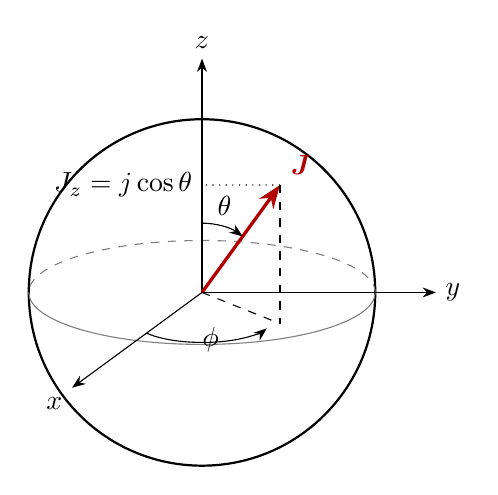
\begin{tikzpicture}[scale=2.2, >=Stealth]
    \draw[thick] (0,0) circle (1);
    \draw[gray] (-1,0) arc (180:360:1 and 0.3);
    \draw[gray,dashed] (1,0) arc (0:180:1 and 0.3);
    \draw[->] (0,0) -- (0,1.35) node[above] {$z$};
    \draw[->] (0,0) -- (-0.75,-0.55) node[below left] {$x$};
    \draw[->] (0,0) -- (1.35,0) node[right] {$y$};
    \coordinate (P) at (0.45,0.62);
    \coordinate (Q) at (0.45,-0.18);
    \draw[->,very thick,red!70!black] (0,0) -- (P) node[above right] {$\vJ$};
    \draw[dashed] (P) -- (Q);
    \draw[dashed] (0,0) -- (Q);
    \draw[->] (0,0.4) arc (90:54:0.4);
    \node at (0.13,0.5) {$\theta$};
    \draw[->] (-0.32,-0.235) arc (216:338:0.4 and 0.13);
    \node at (0.05,-0.27) {$\phi$};
    \draw[dotted] (P) -- (0,0.62) node[left] {$J_z = j\cos\theta$};
  \end{tikzpicture}
  \caption{Coordinates on the phase-space sphere of radius $j$. The canonical pair is $(\phi, J_z)$.}
  \label{fig:sphere-coords}
\end{figure}

\begin{theorem*}
The pair $(q,p) = (\phi, J_z)$ is canonical: $\PB{\phi}{J_z} = 1$.
\end{theorem*}
\begin{proof}
Write $J_x = R\cos\phi$, $J_y = R\sin\phi$ with $R = \sqrt{j^2 - J_z^2}$, so that $\partial R/\partial J_z =
-J_z/R$, and compute brackets with $\PB{A}{B} = \partial_\phi A\,\partial_{J_z}B - \partial_{J_z}A\,\partial_\phi B$, where $\partial_\phi A \equiv
\partial A/\partial\phi$ (the canonical bracket for $q = \phi$, $p = J_z$):
\begin{align*}
  \PB{J_x}{J_y} &= (-R\sin\phi)\Big(-\tfrac{J_z}{R}\sin\phi\Big) - \Big(-\tfrac{J_z}{R}\cos\phi\Big)(R\cos\phi) = J_z, \\
  \PB{J_y}{J_z} &= R\cos\phi = J_x, \qquad \PB{J_z}{J_x} = -(-R\sin\phi) = J_y .
\end{align*}
This reproduces \eqref{eq:J-algebra}, so $(\phi,J_z)$ is a valid canonical pair.
\end{proof}

The phase-space (Liouville) area element is therefore $d\phi\, dJ_z$. The geometric area element of the sphere is
$j^2\sin\theta\, d\theta\, d\phi$, and since $dJ_z = -j\sin\theta\, d\theta$,
\begin{equation}\label{eq:area}
  j^2 \sin\theta\, d\theta\, d\phi = j\; d\phi\, dJ_z .
\end{equation}
\emph{Phase-space area and geometric area on the sphere are the same thing} (up to the constant $j$). This is
Archimedes' ``hat-box'' theorem: the band between two heights $z_1<z_2$ has area proportional to $z_2-z_1$. The total
phase-space area is $4\pi j$. For this reason all phase-space plots in these notes use the axes $(\phi, \cos\theta)$
and not $(\phi,\theta)$: equal areas in the plot are equal areas on the sphere.

\subsection{Linear Hamiltonians generate rotations}\label{sec:precession}

Take $H = \bm\omega\cdot\vJ$ with a constant vector $\bm\omega$. With \eqref{eq:eom-general} and
\eqref{eq:J-f-bracket},
\begin{equation}\label{eq:precession}
  \frac{dJ_i}{dt} = \PB{J_i}{\omega_m J_m} = \epsilon_{imk}\,\omega_m J_k
  \quad\Longleftrightarrow\quad
  \frac{d\vJ}{dt} = \bm\omega \times \vJ .
\end{equation}
This is \emph{precession}. $\vJ$ rotates rigidly about the axis $\hat{\bm\omega} = \bm\omega/|\bm\omega|$ (the unit vector along $\bm\omega$) with angular velocity
$|\bm\omega|$, counter-clockwise when looking down the axis (right-hand rule). After a time $t$ the solution is $\vJ(t) = R_{\hat{\bm\omega}}(|\bm\omega|t)\,\vJ(0)$, where $R_{\hat{\bm n}}(\alpha)$ denotes the $3\times3$ matrix of
a rotation by the angle $\alpha$ about the unit vector $\hat{\bm n}$ (counter-clockwise by the right-hand rule). We
will need the rotations about $y$ and $z$, $R_y \equiv R_{\hat{\bm y}}$ and $R_z \equiv R_{\hat{\bm z}}$, where
$\hat{\bm x} = (1,0,0)$, $\hat{\bm y} = (0,1,0)$, $\hat{\bm z} = (0,0,1)$ are the unit vectors along the axes:
\begin{equation}\label{eq:rotations}
  R_y(\alpha) = \begin{pmatrix} \cos\alpha & 0 & \sin\alpha\\ 0 & 1 & 0 \\ -\sin\alpha & 0 & \cos\alpha \end{pmatrix},
  \qquad
  R_z(\alpha) = \begin{pmatrix} \cos\alpha & -\sin\alpha & 0\\ \sin\alpha & \cos\alpha & 0 \\ 0 & 0 & 1 \end{pmatrix}.
\end{equation}
Check: for $\bm\omega = \hat{\bm y}$, \eqref{eq:precession} gives $\dot\vJ = \hat{\bm y}\times\vJ = (J_z, 0,
-J_x)$, where a dot denotes a time derivative, $\dot\vJ = d\vJ/dt$. Differentiating \eqref{eq:rotations} at $\alpha = 0$
gives the same,
\begin{equation*}
  \frac{d}{d\alpha}R_y(\alpha)\Big|_{\alpha=0}\vJ = \begin{pmatrix}0&0&1\\0&0&0\\-1&0&0\end{pmatrix}\vJ = (J_z, 0, -J_x),
\end{equation*}
and in the same way $\frac{d}{d\alpha}R_z(\alpha)\bm v = \hat{\bm z}\times R_z(\alpha)\bm v$ for any vector $\bm v$.
Rotation matrices are orthogonal, $R^{\mathsf T}R = I$ ($^{\mathsf T}$ is the transpose, $I$ the identity matrix), so
they preserve lengths, $|R\bm v| = |\bm v|$, and $R^{-1} = R^{\mathsf T}$. They also preserve cross products, $R(\bm
a\times\bm b) = (R\bm a)\times(R\bm b)$.

A Hamiltonian that is a function of $\vJ$ but not linear (for example $J_z^2$) still generates a rotation at each
instant, but the axis and the rate depend on where $\vJ$ is. That nonlinearity is the source of chaos.

%---------------------------------------------------------------------
\section{The kicked top}\label{sec:model}

\subsection{Hamiltonian}

The kicked top is an angular momentum $\vJ$ with $|\vJ| = j$ and the time-periodic Hamiltonian
\begin{equation}\label{eq:H}
  \boxed{H(t) = p\, J_y + \frac{k}{2j}\, J_z^2 \sum_{n=-\infty}^{\infty} \delta(t-n) ,}
\end{equation}
with two real parameters:
\begin{itemize}
  \item $p$, the angle of free precession about the $y$ axis accumulated in one period (the period is set to $1$);
  \item $k$, the strength of the \emph{kick}, also called the \emph{torsion} or \emph{twist}.
\end{itemize}
Here $\delta(t)$ is the Dirac delta function: $\delta(t) = 0$ for $t\ne0$, and $\int_a^b f(t)\,\delta(t-t_0)\,dt =
f(t_0)$ for any smooth $f$ and any interval $a < t_0 < b$. The sum $\sum_n\delta(t-n)$ (a \emph{Dirac comb}) switches
the second term on only at the integer times $t = n$, each time as an infinitely short, infinitely strong pulse.
The first term is linear, so it generates a uniform rotation about $y$ (\cref{sec:precession}). The second term acts
only at the instants $t = n$ (integer $n$). It is quadratic in $J_z$: as shown below, it rotates $\vJ$ about the $z$
axis by an angle proportional to $J_z$. Points on the upper hemisphere are turned one way, points on the lower
hemisphere the other way, and the equator not at all, like twisting a towel. The factor $1/j$ makes the twist angle depend only on the
\emph{direction} of $\vJ$ (see below).

Because $H$ depends explicitly on time, \eqref{eq:eom-general} with $A = H$ gives $dH/dt = \PB{H}{H} + \partial
H/\partial t = \partial H/\partial t \ne 0$ (the bracket of anything with itself vanishes), so energy is \emph{not} conserved
(\cref{sec:energy}). With one degree of freedom and no conserved quantity, the motion can be chaotic. In contrast, a
time-independent one-degree-of-freedom system is always integrable.

\subsection{Scaled variables: only the direction matters}\label{sec:scaled}

Since $|\vJ| = j$ is fixed, only the direction of $\vJ$ can change. Introduce the unit vector
\begin{equation}\label{eq:unit}
  \vs = \frac{\vJ}{j} = (X, Y, Z) = (\sin\theta\cos\phi,\ \sin\theta\sin\phi,\ \cos\theta), \qquad |\vs| = 1 .
\end{equation}
Its components are written $s_1 = X$, $s_2 = Y$, $s_3 = Z$ (or $s_x, s_y, s_z$) whenever index notation is
convenient.

\paragraph{The scaled Hamiltonian.} Insert $J_y = jY$ and $J_z = jZ$ into \eqref{eq:H}:
\begin{equation*}
  H = p\,(jY) + \frac{k}{2j}\,(jZ)^2 \sum_n\delta(t-n)
    = j\Big[\,pY + \frac{k}{2}\,Z^2 \sum_n\delta(t-n)\Big].
\end{equation*}
The whole Hamiltonian is $j$ times a function of $\vs$ alone. We write $H = j\,h$ with
\begin{equation}\label{eq:h}
  h(\vs,t) = p\, Y + \frac{k}{2}\, Z^2 \sum_n \delta(t-n).
\end{equation}

\paragraph{The equation of motion for $\vs$.} Let $\nabla_{\!s}$ denote the gradient with respect to the three
components of $\vs$, treated as independent variables:
\begin{equation*}
  \nabla_{\!s}\, h = \Big(\frac{\partial h}{\partial X},\ \frac{\partial h}{\partial Y},\ \frac{\partial h}{\partial Z}\Big),
  \qquad\text{e.g.}\quad \nabla_{\!s}\big(pY\big) = (0, p, 0),\quad \nabla_{\!s}\Big(\frac k2 Z^2\Big) = (0, 0, kZ).
\end{equation*}
Now derive $\dot{\vs}$ in three steps.
\begin{enumerate}
  \item $s_i = J_i/j$ has no explicit time dependence, so by \eqref{eq:eom-general}
  \[ \frac{ds_i}{dt} = \frac1j\,\frac{dJ_i}{dt} = \frac1j\,\PB{J_i}{H}. \]
  \item By \eqref{eq:J-f-bracket} with $f = H$,
  \[ \PB{J_i}{H} = \epsilon_{imk}\,\frac{\partial H}{\partial J_m}\,J_k . \]
  \item $H(\vJ) = j\,h(\vJ/j)$, so by the chain rule $\dfrac{\partial H}{\partial J_m} = j\,\dfrac{\partial h}{\partial
  s_m}\,\dfrac{\partial s_m}{\partial J_m} = j\,\dfrac{\partial h}{\partial s_m}\,\dfrac1j = \dfrac{\partial h}{\partial
  s_m}$, and $J_k = j\,s_k$.
\end{enumerate}
Putting the three together,
\begin{equation*}
  \frac{ds_i}{dt} = \frac1j\,\epsilon_{imk}\,\frac{\partial h}{\partial s_m}\, j\,s_k
                 = \epsilon_{imk}\,\big(\nabla_{\!s} h\big)_m\, s_k ,
\end{equation*}
and the right-hand side is the $i$-th component of the cross product (\cref{sec:angmom}). Hence
\begin{equation}\label{eq:eom-s}
  \boxed{\frac{d\vs}{dt} = \nabla_{\!s}\, h \times \vs .}
\end{equation}
Three remarks.
\begin{itemize}
  \item The radius $j$ has dropped out. The classical dynamics of the direction $\vs$ is the same for every $j$, so we
  can work on the unit sphere. The value of $j$ only matters in the quantum theory, where $1/j$ plays the role of
  Planck's constant (\cref{sec:quantum}).
  \item \eqref{eq:eom-s} keeps $\vs$ on the unit sphere: $\frac{d}{dt}|\vs|^2 = 2\,\vs\cdot\dot{\vs} = 2\,\vs\cdot
  (\nabla_{\!s} h\times\vs) = 0$, because a cross product is perpendicular to each of its factors.
  \item Comparing with \eqref{eq:precession}, \eqref{eq:eom-s} says that at each instant $\vs$ precesses about the
  vector $\bm\omega = \nabla_{\!s} h$, which depends on $\vs$ when $h$ is not linear.
\end{itemize}
For the kicked top \eqref{eq:h},
\begin{equation}\label{eq:grad-h}
  \nabla_{\!s}\, h = p\,\hat{\bm y} + kZ\sum_n \delta(t-n)\,\hat{\bm z} .
\end{equation}

%---------------------------------------------------------------------
\section{The stroboscopic map}\label{sec:map}

Because the Hamiltonian is periodic and the kicks are instantaneous, it is natural to look at the system once per
period, just after each kick. Write $t = n^+$ for the instant just after the kick at $t = n$ and $t = n^-$ for the
instant just before it (the limits from above and from below). Let $\vs_n = \vs(n^+)$. Integrating
\eqref{eq:eom-s} from $t=n^+$ to $t=(n+1)^+$ gives a map $\vs_{n+1} = F(\vs_n)$, the \emph{stroboscopic} or
\emph{Floquet} map. It is derived in two steps: free precession from $n^+$ to $(n+1)^-$, then the kick from
$(n+1)^-$ to $(n+1)^+$.

\paragraph{Step 1: free precession.} For $n < t < n+1$ every $\delta(t-n)$ vanishes, so \eqref{eq:grad-h} is
$\nabla_{\!s} h = p\,\hat{\bm y}$ and \eqref{eq:eom-s} becomes $\dot{\vs} = p\,\hat{\bm y}\times\vs$. With
$\hat{\bm y}\times\vs = (0,1,0)\times(X,Y,Z) = (Z,\ 0,\ -X)$ this is
\begin{equation*}
  \dot X = pZ, \qquad \dot Y = 0, \qquad \dot Z = -pX .
\end{equation*}
$Y$ is constant. Differentiating the first equation and using the third gives $\ddot X = p\dot Z = -p^2X$, a harmonic
oscillator of frequency $p$. With $\tau = t - n$ the time since the kick, and initial values $(X,Y,Z)$ at $\tau=0$,
the solution is
\begin{equation*}
  X(\tau) = X\cos p\tau + Z\sin p\tau, \qquad Z(\tau) = \frac{\dot X(\tau)}{p} = -X\sin p\tau + Z\cos p\tau
\end{equation*}
(check: $X(0) = X$, $Z(0) = Z$, and $\dot Z = -p\,X(\tau)$). At $\tau = 1$, just before the next kick,
\begin{equation}\label{eq:rotation-y}
  X' = X\cos p + Z\sin p, \qquad Y' = Y, \qquad Z' = -X\sin p + Z\cos p ,
\end{equation}
which is $\vs' = R_y(p)\,\vs_n$ with $R_y$ from \eqref{eq:rotations}: a rotation about $y$ by the angle $p$.

\paragraph{Step 2: the kick.} Integrate \eqref{eq:eom-s} over a short interval $[n+1-\varepsilon,\ n+1+\varepsilon]$
and let $\varepsilon\to0$. The precession term $p\,\hat{\bm y}\times\vs$ is bounded (its size is at most $p$), so
its contribution to the change of $\vs$ is at most $2\varepsilon p \to 0$. Only the $\delta$ term survives:
\begin{equation}\label{eq:kick-ode}
  \dot{\vs} = kZ\,\delta(t-n-1)\;\hat{\bm z}\times\vs, \qquad \hat{\bm z}\times\vs = (-Y,\ X,\ 0).
\end{equation}
In components, $\dot Z = 0$, so $Z$ does not change during the kick and keeps its value $Z'$. The other two are
$\dot X = -kZ'\,\delta(t-n-1)\,Y$ and $\dot Y = kZ'\,\delta(t-n-1)\,X$. Introduce the angle accumulated since the start of
the interval,
\begin{equation*}
  \alpha(t) = kZ'\int_{n+1-\varepsilon}^{t}\delta(t''-n-1)\,dt'' ,
\end{equation*}
which rises from $\alpha = 0$ before the kick to $\alpha = kZ'$ after it, with $d\alpha/dt = kZ'\,\delta(t-n-1)$. By
the chain rule $\dot X = (dX/d\alpha)\,\dot\alpha$, so the equations become
\begin{equation*}
  \frac{dX}{d\alpha} = -Y, \qquad \frac{dY}{d\alpha} = X ,
\end{equation*}
a rotation about $z$ with unit rate in $\alpha$: $X = X'\cos\alpha - Y'\sin\alpha$, $Y = X'\sin\alpha + Y'\cos\alpha$.
At the end of the kick, $\alpha = kZ'$:
\begin{equation}\label{eq:torsion}
  X'' = X'\cos(kZ') - Y'\sin(kZ'), \qquad Y'' = X'\sin(kZ') + Y'\cos(kZ'), \qquad Z'' = Z' ,
\end{equation}
i.e.\ $\vs'' = R_z(kZ')\,\vs'$. This is a \emph{torsion}: a rotation about $z$ whose angle depends on the height $Z$.
(Replacing $\delta$ by any narrow pulse of unit area gives the same result, since only the total angle $kZ'$
enters.)

\paragraph{The map.} Together:
\begin{equation}\label{eq:map}
  \boxed{\vs_{n+1} = F(\vs_n) = R_z\!\big(k Z'\big)\, R_y(p)\, \vs_n , \qquad Z' = \big(R_y(p)\vs_n\big)_z .}
\end{equation}
\Cref{fig:map-steps} illustrates the two steps. Two properties follow directly.
\begin{itemize}
  \item Both steps are rotations, which preserve lengths (\cref{sec:precession}), so $|\vs_n| = 1$ holds exactly.
  \item The map is invertible. The torsion does not change $Z$, so the $z$ component of $\vs_{n+1}$ is $Z'$
  itself. Undoing the torsion and then the rotation gives
  \begin{equation*}
    F^{-1}(\vs) = R_y(-p)\,R_z(-kZ)\,\vs ,
  \end{equation*}
  where $Z$ is the $z$ component of the argument $\vs$.
\end{itemize}

\begin{figure}[!htbp]
  \centering
  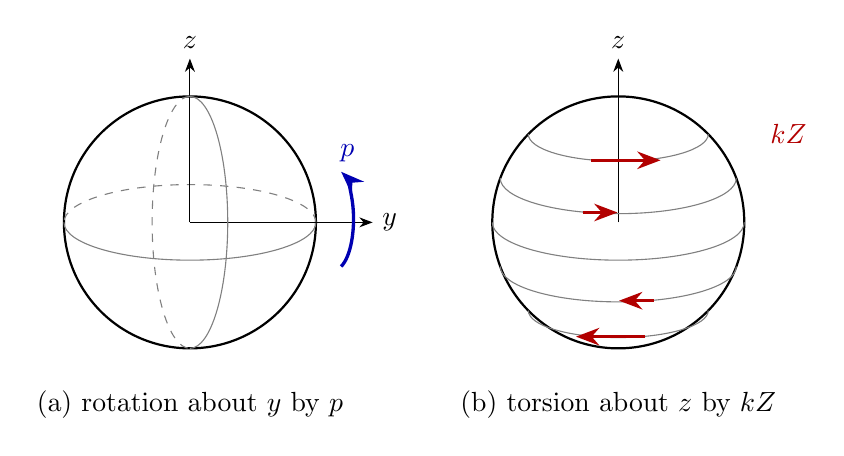
\begin{tikzpicture}[scale=1.6, >=Stealth]
    \begin{scope}
      \draw[thick] (0,0) circle (1);
      \draw[gray] (-1,0) arc (180:360:1 and 0.3);
      \draw[gray,dashed] (1,0) arc (0:180:1 and 0.3);
      \draw[->] (0,0) -- (1.45,0) node[right] {$y$};
      \draw[->] (0,0) -- (0,1.3) node[above] {$z$};
      \draw[gray] (0,-1) arc (-90:90:0.3 and 1);
      \draw[gray,dashed] (0,1) arc (90:270:0.3 and 1);
      \draw[->,very thick,blue!70!black] (1.2,-0.35) arc (-70:70:0.15 and 0.4);
      \node[blue!70!black] at (1.25,0.55) {$p$};
      \node at (0,-1.45) {(a) rotation about $y$ by $p$};
    \end{scope}
    \begin{scope}[xshift=3.4cm]
      \draw[thick] (0,0) circle (1);
      \draw[->] (0,0) -- (0,1.3) node[above] {$z$};
      \foreach \z/\len in {0.7/1, 0.35/0.5, 0/0, -0.35/-0.5, -0.7/-1} {
        \pgfmathsetmacro{\r}{sqrt(1-\z*\z)}
        \draw[gray] (-\r,\z) arc (180:360:\r cm and 0.3*\r cm);
        \ifdim \len pt > 0pt
          \draw[->,very thick,red!70!black] (-0.3*\r,\z-0.29*\r) -- ++(0.55*\len,0);
        \fi
        \ifdim \len pt < 0pt
          \draw[->,very thick,red!70!black] (0.3*\r,\z-0.29*\r) -- ++(0.55*\len,0);
        \fi
      }
      \node[red!70!black] at (1.35,0.7) {$kZ$};
      \node at (0,-1.45) {(b) torsion about $z$ by $kZ$};
    \end{scope}
  \end{tikzpicture}
  \caption{The two steps of one period of the kicked top, \cref{eq:map}. (a) A rigid rotation about $y$. (b) A
  rotation about $z$ whose angle $kZ$ grows with height: the upper and lower hemispheres are twisted in opposite
  directions and the equator stays put.}
  \label{fig:map-steps}
\end{figure}

\subsection{The map preserves phase-space area}\label{sec:area}

If a map sends coordinates $(q,P)$ to $(q'', P'')$, a small area element is multiplied by $|\det D|$, where $D$ is
the \emph{Jacobian matrix} of partial derivatives
\begin{equation*}
  D = \begin{pmatrix} \partial q''/\partial q & \partial q''/\partial P\\ \partial P''/\partial q & \partial P''/\partial P\end{pmatrix}
\end{equation*}
and $\det$ is its determinant. We use the canonical coordinates $(\phi, Z)$ of \cref{sec:canonical}.

\paragraph{The torsion.} With $X = \sqrt{1-Z^2}\cos\phi$ and $Y = \sqrt{1-Z^2}\sin\phi$ (from \eqref{eq:unit}), the
rotation \eqref{eq:torsion} by the angle $\alpha$ reads, using the addition formulas for $\cos$ and $\sin$,
\begin{equation*}
  X'' = \sqrt{1-Z'^2}\,\cos(\phi'+\alpha), \qquad Y'' = \sqrt{1-Z'^2}\,\sin(\phi'+\alpha), \qquad Z'' = Z' .
\end{equation*}
So a rotation about $z$ only shifts $\phi$ by $\alpha$. With $\alpha = kZ'$,
\begin{equation}\label{eq:twist}
  \phi'' = \phi' + kZ', \qquad Z'' = Z' ,
  \qquad
  D_{\rm torsion} = \begin{pmatrix} \partial\phi''/\partial\phi' & \partial\phi''/\partial Z'\\ \partial Z''/\partial\phi' & \partial Z''/\partial Z'\end{pmatrix}
  = \begin{pmatrix}1 & k\\ 0 & 1\end{pmatrix},
\end{equation}
and $\det D_{\rm torsion} = 1\cdot1 - k\cdot0 = 1$. A map of this form, where one coordinate is shifted by an amount
that grows with the other, is called a \emph{twist map}.

\paragraph{The rotation.} $R_y(p)$ moves the sphere rigidly, so it preserves geometric area on the sphere. By
\eqref{eq:area} geometric area and phase-space area $d\phi\,dZ$ are the same, so $|\det D_{\rm rotation}| = 1$. (The
same follows from Liouville's theorem, since $R_y(p)$ is the flow of the Hamiltonian $pY$.)

\paragraph{The full map.} By the chain rule the Jacobian of a composition is the product of the Jacobians, and
$\det(AB) = \det A\,\det B$. Hence
\begin{equation}
  \det DF = \det D_{\rm torsion}\,\det D_{\rm rotation} = 1 \quad\text{(in the coordinates $(\phi,Z)$)}.
\end{equation}
(The coordinates $(\phi,Z)$ fail at the poles $Z=\pm1$, where $\phi$ is undefined, but that is a property of the
coordinates and not of the map.) Two consequences will be used repeatedly. First, there are no attractors: a region of
phase space can be stretched and folded but never shrunk. Second, linear stability is decided by a single number,
the trace of the Jacobian (\cref{sec:stability}).

%---------------------------------------------------------------------
\section{Energy}\label{sec:energy}

The code evaluates, at every recorded point $\vs_n$, the two terms of the scaled Hamiltonian \eqref{eq:h} without the
$\delta$ comb, and their sum:
\begin{equation}\label{eq:energy}
  E_{\rm rot} = pY, \qquad E_{\rm kick} = \frac{k}{2}Z^2, \qquad E = E_{\rm rot} + E_{\rm kick} = pY + \frac{k}{2}Z^2 .
\end{equation}
For $p, k \ge 0$, $|Y|\le1$ and $0\le Z^2\le1$ give $-p \le E \le p + k/2$. The minimum $E = -p$ is reached at
$-\hat{\bm y}$, where $Y=-1$ and $Z=0$.

\paragraph{Why $E$ is not conserved.} Follow $E$ through one period with \eqref{eq:rotation-y} and \eqref{eq:torsion}.
\begin{itemize}
  \item During the precession $Y$ is constant, so $E_{\rm rot}$ is unchanged, but $Z \to Z' = -X\sin p + Z\cos p$
  changes $E_{\rm kick}$.
  \item During the kick $Z$ is constant, so $E_{\rm kick}$ is unchanged, but $Y \to Y'' = X'\sin(kZ') + Y'\cos(kZ')$
  changes $E_{\rm rot}$.
\end{itemize}
Over one period
\begin{equation*}
  E_{n+1} - E_n = p\,\big(Y'' - Y\big) + \frac k2\big(Z'^2 - Z^2\big),
\end{equation*}
which is not zero in general. This is the explicit form of $dH/dt = \partial H/\partial t \ne 0$
(\cref{sec:model}). There are, however, two reasons why $E$ is a useful quantity.

\paragraph{The near-continuous limit.} Suppose both $p$ and $k$ are small. Expand both steps to first order. A
rotation by a small angle $\alpha$ about $\hat{\bm n}$ is $R_{\hat{\bm n}}(\alpha)\vs = \vs + \alpha\,\hat{\bm n}
\times\vs + O(\alpha^2)$ (the derivative of the rotation at $\alpha = 0$, as checked in \cref{sec:precession}).
So
\begin{align*}
  \vs' &= \vs + p\,\hat{\bm y}\times\vs + O(p^2), \\
  \vs_{n+1} &= \vs' + kZ'\,\hat{\bm z}\times\vs' + O(k^2) = \vs + \big(p\,\hat{\bm y} + kZ\,\hat{\bm z}\big)\times\vs
  + O(p^2, pk, k^2),
\end{align*}
where we used $Z' = Z + O(p)$ and $\vs' = \vs + O(p)$. Now $p\,\hat{\bm y} + kZ\,\hat{\bm z} = (0,\, p,\, kZ) =
\nabla_{\!s}\,h_{\rm eff}$ with the \emph{effective Hamiltonian}
\begin{equation}\label{eq:heff}
  h_{\rm eff} = pY + \frac{k}{2}Z^2 = E .
\end{equation}
So $\vs_{n+1} = \vs_n + \nabla_{\!s} h_{\rm eff}\times\vs_n + O(p^2, pk, k^2)$: one period is, to first order, a step
of length $1$ of the continuous motion $\dot{\vs} = \nabla_{\!s} h_{\rm eff}\times\vs$. (The Baker--Campbell--Hausdorff
formula makes this systematic: the exact time-$1$ flow of $h_{\rm eff}$ and the map $F$ differ only at order $pk$.)
The flow of a time-independent Hamiltonian conserves it:
\begin{equation*}
  \frac{d h_{\rm eff}}{dt} = \nabla_{\!s} h_{\rm eff}\cdot\dot{\vs} = \nabla_{\!s} h_{\rm eff}\cdot\big(\nabla_{\!s}
  h_{\rm eff}\times\vs\big) = 0 .
\end{equation*}
So in this limit $E$ is nearly conserved and orbits follow the level curves of $E$. \Cref{fig:near-flow} shows this
for $p = 0.1$, $k = 0.2$: every orbit traces a curve of (almost) constant colour.

\paragraph{Fixed points of the effective flow.} The flow stops where $\dot{\vs} = \nabla_{\!s} h_{\rm eff}\times\vs =
0$, i.e.\ where $\nabla_{\!s} h_{\rm eff}$ is parallel to $\vs$: $\nabla_{\!s} h_{\rm eff} = \mu\,\vs$ for some
number $\mu$. (This is also the Lagrange condition for the extrema of $h_{\rm eff}$ on the sphere, with $\mu$ the
Lagrange multiplier.) In components,
\begin{equation*}
  0 = \mu X, \qquad p = \mu Y, \qquad kZ = \mu Z .
\end{equation*}
For $p\ne0$ the second equation forces $\mu\ne0$, so the first gives $X = 0$. The third has two solutions.
\begin{itemize}
  \item $Z = 0$: then $Y = \pm1$, the poles $\pm\hat{\bm y}$.
  \item $\mu = k$: then $Y = p/k$ and $Z = \pm\sqrt{1 - p^2/k^2}$, which exists only if $k \ge p$.
\end{itemize}
For $p=0.1$, $k=0.2$ the second pair is at $Y = 0.5$, $X = 0$, i.e.\ $\phi = \pi/2$, $Z = \pm0.87$: the two centres
visible in \cref{fig:near-flow}.

To see which points are centres and which are saddles, expand $h_{\rm eff}$ near $\sigma\hat{\bm y}$
($\sigma = \pm1$) with small $x = X$, $z = Z$. From $Y = \sigma\sqrt{1 - x^2 - z^2} \approx \sigma\big(1 - \tfrac12(x^2
+ z^2)\big)$,
\begin{equation*}
  h_{\rm eff} \approx \sigma p - \frac{\sigma p}{2}\,x^2 + \frac{k - \sigma p}{2}\,z^2 .
\end{equation*}
At $-\hat{\bm y}$ ($\sigma=-1$) both coefficients are positive, so $h_{\rm eff}$ has a minimum there. Its level curves
are small closed curves around the point, so it is a \emph{centre}. At $+\hat{\bm y}$ the coefficients are $-p/2$
and $(k-p)/2$. For $k<p$ both are negative (a maximum, a centre). For $k>p$ they have opposite signs, the level curves
are hyperbolas, and $+\hat{\bm y}$ is a \emph{saddle}: orbits approach it along one direction and leave along
another. This is the case in \cref{fig:near-flow} ($\phi = \pi/2$, $Z = 0$), where the curve through the saddle (the
\emph{separatrix}) is clearly visible.

\begin{figure}[!htbp]
  \centering
  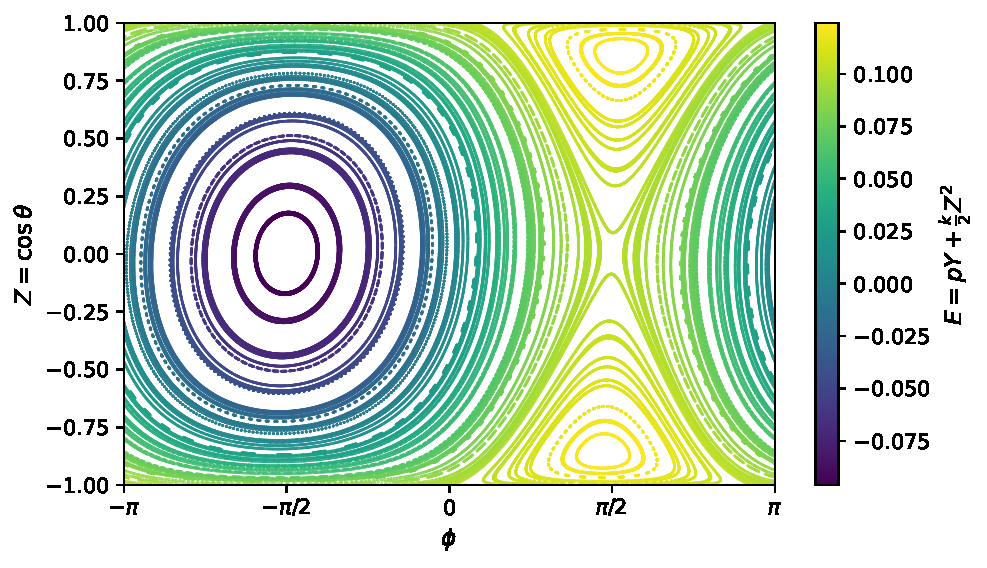
\includegraphics[width=0.75\textwidth]{figures/near_flow.pdf}
  \caption{Phase portrait for small parameters $p = 0.1$, $k = 0.2$ ($12\times12$ grid of initial conditions, $1000$
  kicks each), coloured by $E$ of \cref{eq:energy}. Orbits lie on level curves of $E$, as predicted by \cref{eq:heff}.}
  \label{fig:near-flow}
\end{figure}

\paragraph{Away from that limit.} For $p = \pi/2$ the near-continuous picture does not apply and $E$ fluctuates from
kick to kick (\cref{fig:energy}). On a regular orbit (left) the fluctuations are quasi-periodic and stay inside a narrow
band. On a chaotic orbit (right) they are erratic, and $E$ wanders over a large part of its range $[-p,\ p + k/2]$. The
behaviour of $E_n$ is thus a simple diagnostic of regular versus chaotic motion.

\begin{figure}[!htbp]
  \centering
  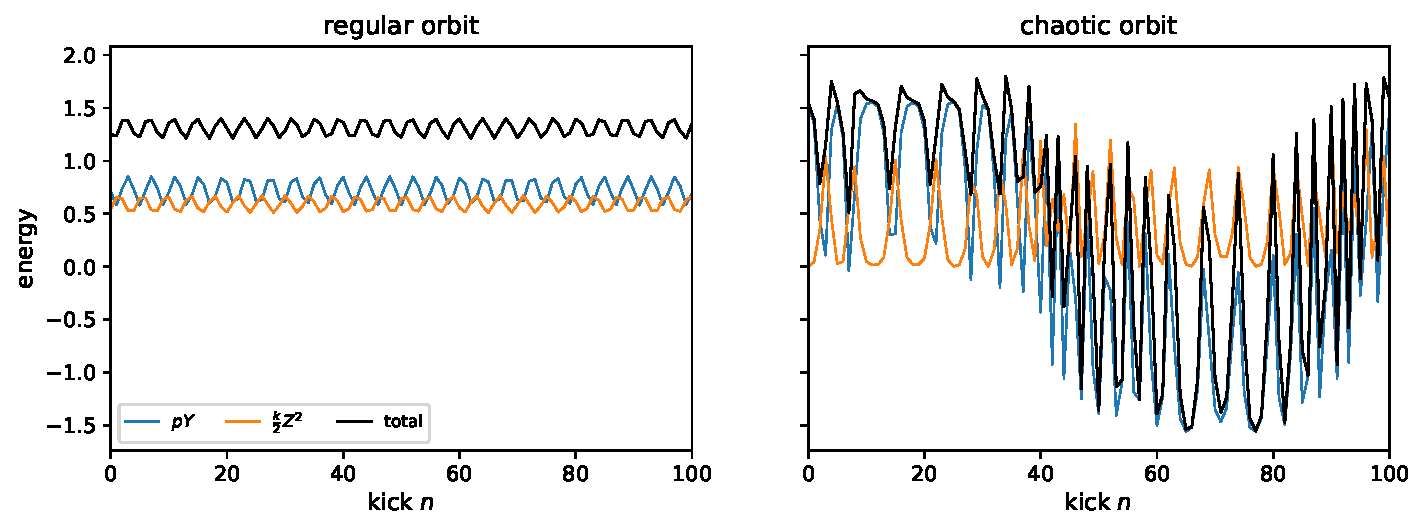
\includegraphics[width=\textwidth]{figures/energy.pdf}
  \caption{The energy terms \eqref{eq:energy} along a regular orbit (left, started inside the island around the fixed
  point $\vs_+$ of \cref{sec:pi2}) and along a chaotic orbit (right, started next to the unstable pole $+\hat{\bm y}$),
  for $p = \pi/2$, $k = 3$.}
  \label{fig:energy}
\end{figure}

%---------------------------------------------------------------------
\section{Integrable limits and symmetry}\label{sec:symmetry}

\paragraph{Integrable limits.} A map is called \emph{integrable} if there is a conserved function $I(\vs)$,
$I(F(\vs)) = I(\vs)$. Each orbit then stays on one level curve $I = $ const, an \emph{invariant curve}.
\begin{itemize}
  \item $k = 0$: the torsion is $R_z(0)$, the identity, and $F = R_y(p)$. $Y$ is conserved. Every orbit lies on a
  circle $Y = $ const and advances by the angle $p$ per kick. If $p/2\pi = r/q$ with integers $r, q$, then
  $R_y(p)^q = R_y(2\pi r)$ is the identity and every orbit is periodic with period $q$ (for $p = \pi/2$, $q = 4$).
  \item $p = 0$: $F$ is the pure twist \eqref{eq:twist} and $Z$ is conserved. Each circle of latitude rotates rigidly
  by its own angle, $\phi_n = \phi_0 + n\,kZ$.
\end{itemize}
When both $p$ and $k$ are non-zero there is in general no conserved quantity.

\paragraph{A symmetry.} Let $S = R_y(\pi)$. From \eqref{eq:rotations} with $\cos\pi = -1$, $\sin\pi = 0$,
\begin{equation*}
  S = \begin{pmatrix}-1&0&0\\0&1&0\\0&0&-1\end{pmatrix}, \qquad (X,Y,Z)\mapsto(-X,\ Y,\ -Z), \qquad S^{-1} = S .
\end{equation*}
We show that $F(S\vs) = S\,F(\vs)$.
\begin{enumerate}
  \item Rotations about the same axis commute, $R_y(\pi)R_y(p) = R_y(\pi+p) = R_y(p)R_y(\pi)$. So $R_y(p)\,S\vs =
  S\,\vs'$ with $\vs' = R_y(p)\vs$.
  \item $S$ flips the sign of the $z$ component, so the torsion angle for $S\vs'$ is $-kZ'$. Hence $F(S\vs) =
  R_z(-kZ')\,S\,\vs'$.
  \item Multiply out $S R_z(\alpha) S$ with \eqref{eq:rotations}: each entry $(R_z)_{ab}$ gets the factor $S_{aa}
  S_{bb}$, which flips the sign of the two $\sin\alpha$ entries and nothing else. So $S R_z(\alpha) S = R_z(-\alpha)$,
  or $R_z(-\alpha)\,S = S\,R_z(\alpha)$.
  \item With $\alpha = kZ'$: $F(S\vs) = R_z(-kZ')\,S\,\vs' = S\,R_z(kZ')\,\vs' = S\,F(\vs)$.
\end{enumerate}
The two sign changes (of the axis and of the height) cancel:
\begin{equation}\label{eq:symmetry}
  F(S\vs) = S\,F(\vs) .
\end{equation}
If $\vs_0, \vs_1, \dots$ is an orbit, then $S\vs_{n+1} = S F(\vs_n) = F(S\vs_n)$, so $S\vs_0, S\vs_1, \dots$ is also an
orbit. In the coordinates $(\phi, Z)$, $S$ is $(\phi, Z)\mapsto(\pi-\phi, -Z)$, since $\cos(\pi-\phi) = -\cos\phi$ and
$\sin(\pi-\phi) = \sin\phi$. This is a point reflection about $(\pi/2, 0)$ (with $\phi$ taken modulo $2\pi$), and every
phase portrait in these notes is symmetric under it. Orbits either come in symmetric pairs or are symmetric
themselves.

%---------------------------------------------------------------------
\section{Fixed points, periodic orbits and their stability}\label{sec:stability}

\subsection{Linear stability of an area-preserving map}

A point $\vs^*$ with $F(\vs^*) = \vs^*$ is a \emph{fixed point}. A point with $F^m(\vs^*) = \vs^*$, where $F^m = F\circ
\dots\circ F$ is $F$ applied $m$ times and $m$ is the smallest such number, lies on a \emph{periodic orbit} of period
$m$.

\paragraph{Linearisation.} To see what happens near $\vs^*$, write $\vs = \vs^* + \delta\vs$, where $\delta\vs$ (here
$\delta$ means ``a small change of'', not the Dirac function) is small. Since $|\vs| = |\vs^*| = 1$, to first order
$\vs^*\cdot\delta\vs = 0$: $\delta\vs$ lies in the \emph{tangent plane} of the sphere at $\vs^*$. Choose two orthogonal
unit vectors $\hat{\bm e}_1, \hat{\bm e}_2$ spanning that plane and write $\delta\vs = a_1\hat{\bm e}_1 + a_2\hat{\bm
e}_2$. A Taylor expansion of $F$ to first order gives
\begin{equation}
  F(\vs^* + \delta\vs) = \vs^* + M\,\delta\vs + O(\delta\vs^2)
  \qquad\Longrightarrow\qquad
  \delta\vs_{n+1} = M\,\delta\vs_n ,
\end{equation}
where $M$ is the $2\times2$ Jacobian matrix $DF(\vs^*)$ in the basis $(\hat{\bm e}_1, \hat{\bm e}_2)$: its entry $M_{ab}$
is the $\hat{\bm e}_a$ component of the change of $F$ when $\vs^*$ is moved by a unit amount along $\hat{\bm e}_b$. For a
period-$m$ orbit $\vs^*_0\to\vs^*_1\to\dots\to\vs^*_m = \vs^*_0$ the chain rule gives the product of the Jacobians along
the orbit, $M^{(m)} = DF(\vs^*_{m-1})\cdots DF(\vs^*_1)\,DF(\vs^*_0)$.

\paragraph{The trace decides.} The trace $\Tr M = M_{11} + M_{22}$ and the determinant $\det M$ do not depend on the
basis: a change of basis replaces $M$ by $PMP^{-1}$, and $\Tr(PMP^{-1}) = \Tr M$, $\det(PMP^{-1}) = \det M$. Area
preservation (\cref{sec:area}) gives $\det M = 1$. The eigenvalues $\lambda$ of $M$ ($M\bm v = \lambda\bm v$ for some
vector $\bm v\ne0$) solve
\begin{equation*}
  \det(M - \lambda I) = \lambda^2 - (\Tr M)\,\lambda + \det M = \lambda^2 - (\Tr M)\,\lambda + 1 = 0,
  \qquad
  \lambda_{1,2} = \frac{\Tr M \pm \sqrt{(\Tr M)^2 - 4}}{2},
\end{equation*}
with $\lambda_1\lambda_2 = 1$. Three cases:
\begin{itemize}
  \item $|\Tr M| < 2$: \textbf{elliptic} (stable). The square root is imaginary, $\lambda_{1,2} = e^{\pm i\alpha}$ with
  $\lambda_1 + \lambda_2 = 2\cos\alpha = \Tr M$. In a suitable basis $M$ acts as a rotation by $\alpha$, so nearby
  points circle around $\vs^*$ by about $\alpha$ per kick on small ellipses and stay close. In the phase portrait an
  elliptic point sits at the centre of a family of closed curves, an \emph{island}.
  \item $|\Tr M| > 2$: \textbf{hyperbolic} (unstable). Two real eigenvalues $\lambda_u$ and $1/\lambda_u$ with
  $|\lambda_u| > 1$. A displacement along the eigenvector of $\lambda_u$ grows like $|\lambda_u|^n$, one along the other
  eigenvector shrinks like $|\lambda_u|^{-n}$. Hyperbolic points are the seeds of chaos.
  \item $|\Tr M| = 2$: \textbf{parabolic}, $\lambda_1 = \lambda_2 = \pm1$. This is the boundary case at which
  \textbf{bifurcations} happen. At $\Tr M = +2$ ($\lambda = 1$) new fixed points can branch off. At $\Tr M = -2$
  ($\lambda = -1$) a displacement flips sign every kick and comes back after two, and the fixed point typically gives
  birth to a period-2 orbit (\emph{period doubling}).
\end{itemize}

\subsection{The poles \texorpdfstring{$\pm\hat{\bm y}$}{+-y}}\label{sec:poles}

The two points $\vs = \sigma\hat{\bm y}$, $\sigma = \pm1$, are fixed for all $p$ and $k$. $R_y(p)$ leaves them alone,
because they lie on its axis. Then $Z' = 0$, so the torsion angle $kZ'$ is zero and the torsion does nothing.

Near $\sigma\hat{\bm y}$ write $\vs = (x,\ \sigma\sqrt{1-x^2-z^2},\ z) \approx (x,\ \sigma,\ z)$ with small $x, z$. The
tangent plane is spanned by $\hat{\bm x}, \hat{\bm z}$, and $(x, z)$ are the coordinates in it.
\begin{itemize}
  \item The rotation \eqref{eq:rotation-y} acts on $(x,z)$ as $x' = x\cos p + z\sin p$, $z' = -x\sin p + z\cos p$.
  \item The torsion \eqref{eq:torsion} with $X' = x'$, $Y' \approx \sigma$ and the small angle $kz'$
  ($\cos kz'\approx1$, $\sin kz'\approx kz'$) gives $x'' \approx x' - \sigma kz'$, $z'' = z'$, dropping products of small
  quantities.
\end{itemize}
Hence
\begin{equation}
  M_\sigma = \begin{pmatrix}1 & -\sigma k\\ 0 & 1\end{pmatrix}\begin{pmatrix}\cos p & \sin p\\ -\sin p & \cos p\end{pmatrix}
           = \begin{pmatrix} \cos p + \sigma k \sin p & \sin p - \sigma k\cos p\\ -\sin p & \cos p\end{pmatrix},
\end{equation}
with $\det M_\sigma = (\cos p + \sigma k\sin p)\cos p + \sin p\,(\sin p - \sigma k\cos p) = \cos^2p + \sin^2p = 1$ and
\begin{equation}\label{eq:pole-trace}
  \boxed{\Tr M_\sigma = 2\cos p + \sigma\, k \sin p .}
\end{equation}
For $p = \pi/2$ ($\cos p = 0$, $\sin p = 1$) this is $\Tr M_\pm = \pm k$. Both poles are stable for $k<2$, and both
become unstable at $k = 2$: $+\hat{\bm y}$ through $\Tr = +2$ and $-\hat{\bm y}$ through $\Tr = -2$. For small $p$,
$\cos p \approx 1 - p^2/2$ and $\sin p \approx p$ give $\Tr M_+ \approx 2 - p^2 + kp$, which exceeds $2$ when $k > p$:
the same threshold at which $+\hat{\bm y}$ became a saddle of $h_{\rm eff}$ in \cref{sec:energy}.

\subsection{The case \texorpdfstring{$p = \pi/2$}{p = pi/2}}\label{sec:pi2}

From now on we use the standard choice $p = \pi/2$. With $\cos p = 0$, $\sin p = 1$, \eqref{eq:rotation-y} becomes
$(X', Y', Z') = (Z,\ Y,\ -X)$. The torsion angle is $kZ' = -kX$, and with $\cos(-kX) = \cos kX$, $\sin(-kX) = -\sin
kX$, \eqref{eq:torsion} gives
\begin{equation}\label{eq:map-pi2}
  X_{n+1} = Z_n\cos(kX_n) + Y_n\sin(kX_n), \quad
  Y_{n+1} = -Z_n\sin(kX_n) + Y_n\cos(kX_n), \quad
  Z_{n+1} = -X_n .
\end{equation}

\paragraph{The fixed points born at $k=2$.} A fixed point needs $Z_{n+1} = Z_n$, i.e.\ $Z = -X$. Write $a = kX$ and
insert $Z = -X$ into the first two equations of \eqref{eq:map-pi2}, using $1 + \cos a = 2\cos^2\frac a2$, $1 - \cos a =
2\sin^2\frac a2$ and $\sin a = 2\sin\frac a2\cos\frac a2$:
\begin{align*}
  X = -X\cos a + Y\sin a \;&\Longrightarrow\; X(1+\cos a) = Y\sin a \;\Longrightarrow\; X\cos\tfrac a2 = Y\sin\tfrac a2, \\
  Y = X\sin a + Y\cos a \;&\Longrightarrow\; Y(1-\cos a) = X\sin a \;\Longrightarrow\; Y\sin\tfrac a2 = X\cos\tfrac a2 .
\end{align*}
Both give the same condition $Y = X\cot(kX/2)$. ($X = 0$ gives $Z = 0$, $Y=\pm1$: the poles again.) The normalisation
$X^2 + Y^2 + Z^2 = 1$ then gives
\begin{equation}\label{eq:fp}
  g(X) \equiv 2X^2 + X^2\cot^2\!\Big(\frac{kX}{2}\Big) = 1, \qquad \vs_\pm = \big(\pm X,\ X\cot(kX/2),\ \mp X\big).
\end{equation}
$X\cot(kX/2)$ is even in $X$, so the solutions come in pairs $\pm X$ with the same $Y$. For small $u$, $\cot u \approx
1/u$, so $X\cot(kX/2) \to 2/k$ and $g(X) \to 4/k^2$ as $X\to0$.
\begin{itemize}
  \item $k < 2$: $g(0) = 4/k^2 > 1$, and a numerical scan confirms that $g(X) = 1$ has no solution.
  \item $k = 2$: $g(0) = 1$, the solution sits at $X = 0$, $Y = 2/k = 1$, i.e.\ at the pole $+\hat{\bm y}$.
  \item $k > 2$: a pair $\vs_\pm$ with small $X$ moves away from $+\hat{\bm y}$.
\end{itemize}
So $\vs_\pm$ branch off the pole $+\hat{\bm y}$ exactly at $k = 2$, where the pole's trace passes $+2$: a
\emph{pitchfork bifurcation} (one fixed point becomes three). The two points are mapped onto each other by $S$ of
\eqref{eq:symmetry}: $S(X, Y, -X) = (-X, Y, X)$. Solving \eqref{eq:fp} numerically and computing the trace of the
Jacobian of \eqref{eq:map-pi2} in the tangent plane:

\begin{center}
\begin{tabular}{cccc}
\toprule
$k$ & $\vs_+ = (X,Y,Z)$ & $(\phi, Z)$ & $\Tr M$ \\
\midrule
2.5 & $(0.514,\ 0.687,\ -0.514)$ & $(0.928,\ -0.514)$ & $\phantom{-}1.00$ \\
3.0 & $(0.629,\ 0.456,\ -0.629)$ & $(0.627,\ -0.629)$ & $\phantom{-}0.06$ \\
3.5 & $(0.681,\ 0.272,\ -0.681)$ & $(0.380,\ -0.681)$ & $-0.77$ \\
4.0 & $(0.702,\ 0.118,\ -0.702)$ & $(0.167,\ -0.702)$ & $-1.47$ \\
\bottomrule
\end{tabular}
\end{center}

\paragraph{Period doubling of $\vs_\pm$ at $k = \pi\sqrt2$.} The trace decreases with $k$ and reaches $-2$ at $k =
\pi\sqrt2 \approx 4.443$. This can be checked exactly. At $k = \pi\sqrt2$ and $X = 1/\sqrt2$, $kX/2 = \pi/2$ and
$\cot(\pi/2) = 0$, so $Y = 0$ and $g = 2\cdot\frac12 = 1$: \eqref{eq:fp} is solved by $\vs_+ = (1, 0, -1)/\sqrt2$.
Its tangent plane is spanned by $\hat{\bm u} = \hat{\bm y}$ and $\hat{\bm w} = (\hat{\bm x}+\hat{\bm z})/\sqrt2$.
Write $\vs = \vs_+ + a\,\hat{\bm u} + b\,\hat{\bm w}$:
\begin{equation*}
  X = \frac{1+b}{\sqrt2}, \qquad Y = a, \qquad Z = \frac{-1+b}{\sqrt2}, \qquad kX = \pi(1+b),
\end{equation*}
so to first order $\cos kX = -\cos\pi b \approx -1$ and $\sin kX = -\sin\pi b \approx -\pi b$. Inserting into
\eqref{eq:map-pi2} and dropping products of $a, b$:
\begin{equation*}
  X_{n+1} \approx \frac{1-b}{\sqrt2}, \qquad Y_{n+1} \approx -\frac{\pi}{\sqrt2}\,b - a, \qquad Z_{n+1} = -\frac{1+b}{\sqrt2},
\end{equation*}
i.e.\ $\vs_{n+1} = \vs_+ + a'\hat{\bm u} + b'\hat{\bm w}$ with $a' = -a - \frac{\pi}{\sqrt2}b$, $b' = -b$. Hence
\begin{equation*}
  M = \begin{pmatrix} -1 & -\pi/\sqrt2\\ 0 & -1\end{pmatrix}, \qquad \det M = 1, \qquad \Tr M = -2 .
\end{equation*}
Beyond $k\approx4.44$ the fixed points $\vs_\pm$ are unstable (period doubling), and their islands disappear from the
phase portraits (\cref{fig:portraits}, $k = 4.5$).

\paragraph{A period-2 orbit born at $k = 2$.} At $k=2$ the pole $-\hat{\bm y}$ passes $\Tr = -2$ and, by the period
doubling scenario of \cref{sec:stability}, emits a period-2 orbit: two points $\vs_A, \vs_B$ with $F(\vs_A) = \vs_B$,
$F(\vs_B) = \vs_A$. For $k = 3$ a numerical search gives $(\phi, Z) = (-0.627,\ 0.629)$ and $(-2.515,\ -0.629)$, with
$\Tr M^{(2)} = \Tr\big[DF(\vs_B)\,DF(\vs_A)\big] = -1.93$ (stable, close to its own period doubling).

\paragraph{A period-4 orbit for every $k$.} Follow $\hat{\bm x}$ under \eqref{eq:map-pi2}, using $R_y(\pi/2):
(X,Y,Z)\mapsto(Z,Y,-X)$:
\begin{gather*}
  \hat{\bm x} \xrightarrow{R_y} -\hat{\bm z} \xrightarrow{\text{torsion}} -\hat{\bm z}, \qquad
  -\hat{\bm z} \xrightarrow{R_y} -\hat{\bm x} \xrightarrow{\text{torsion}} -\hat{\bm x}, \\
  -\hat{\bm x} \xrightarrow{R_y} \hat{\bm z} \xrightarrow{\text{torsion}} \hat{\bm z}, \qquad
  \hat{\bm z} \xrightarrow{R_y} \hat{\bm x} \xrightarrow{\text{torsion}} \hat{\bm x}.
\end{gather*}
After each rotation the point lies either on the $z$ axis (which a rotation about $z$ does not move) or on the
equator (where the torsion angle is zero). So $\hat{\bm x} \to -\hat{\bm z} \to -\hat{\bm x} \to \hat{\bm z} \to
\hat{\bm x}$ is a period-4 orbit for every $k$.

Its stability needs the linearised torsion. Differentiate $T(\vs) = R_z(kZ)\,\vs$, using the derivative of
$R_z$ from \cref{sec:precession}:
\begin{equation*}
  DT(\vs)\,\delta\vs = R_z(kZ)\,\delta\vs + k\,\delta Z\;\hat{\bm z}\times R_z(kZ)\,\vs .
\end{equation*}
At the poles $\pm\hat{\bm z}$ the second term vanishes ($\hat{\bm z}\times\hat{\bm z} = 0$) and the torsion acts on the
tangent plane as the rotation $R_z(\pm k)$. On the equator at $\pm\hat{\bm x}$, $R_z(0) = I$ and $\hat{\bm z}\times
(\pm\hat{\bm x}) = \pm\hat{\bm y}$, so $DT\,\delta\vs = \delta\vs \pm k\,\delta Z\,\hat{\bm y}$, a shear. Use the
tangent bases $(\hat{\bm y}, \hat{\bm z})$ at $\pm\hat{\bm x}$ and $(\hat{\bm x}, \hat{\bm y})$ at $\pm\hat{\bm z}$.
Following a displacement through $R_y(\pi/2)$ ($\hat{\bm y}\to\hat{\bm y}$, $\hat{\bm z}\to\hat{\bm x}$, $\hat{\bm
x}\to-\hat{\bm z}$) and then the torsion gives the four $2\times2$ Jacobians
\begin{align*}
  \hat{\bm x}\to-\hat{\bm z}:\ D_1 &= \begin{pmatrix}\sin k & \cos k\\ \cos k & -\sin k\end{pmatrix}, &
  -\hat{\bm z}\to-\hat{\bm x}:\ D_2 &= \begin{pmatrix}k & 1\\ -1 & 0\end{pmatrix}, \\
  -\hat{\bm x}\to\hat{\bm z}:\ D_3 &= \begin{pmatrix}-\sin k & \cos k\\ \cos k & \sin k\end{pmatrix}, &
  \hat{\bm z}\to\hat{\bm x}:\ D_4 &= \begin{pmatrix}-k & 1\\ -1 & 0\end{pmatrix}.
\end{align*}
(The bases are not all oriented the same way, so $\det D_1 = \det D_3 = -1$. Only the product is meaningful, and it
has determinant $1$.) Multiplying out $M^{(4)} = D_4 D_3 D_2 D_1$ and simplifying with $\cos^2k - \sin^2k = \cos2k$,
$2\sin k\cos k = \sin 2k$,
\begin{equation}\label{eq:period4-trace}
  \boxed{\Tr M^{(4)} = 2\cos 2k + 2k\sin 2k + k^2\sin^2 k .}
\end{equation}
For small $k$, $\Tr M^{(4)} = 2 - k^4/3 + O(k^6)$, just below $2$ (marginally stable). The trace depends on $k$ in a
non-monotonic way:
\begin{center}
\begin{tabular}{ccccccc}
\toprule
$k$ & 0.5 & 1.5 & 2.5 & 3.0 & 4.5 & 6.0\\
\midrule
$\Tr M^{(4)}$ & 1.98 & 0.68 & $-1.99$ & 0.42 & 21.2 & $-1.94$ \\
\bottomrule
\end{tabular}
\end{center}
These values agree with a direct numerical evaluation of the Jacobians. The orbit is stable at $k = 3$ and at $k = 6$:
its islands are visible around $(\phi,Z) = (0,0)$, $(\pm\pi, 0)$ and near the poles $Z = \pm1$ in
\cref{fig:portraits}. At $k = 4.5$ it is unstable.

%---------------------------------------------------------------------
\section{From regular to chaotic motion}\label{sec:chaos}

\begin{figure}[!htbp]
  \centering
  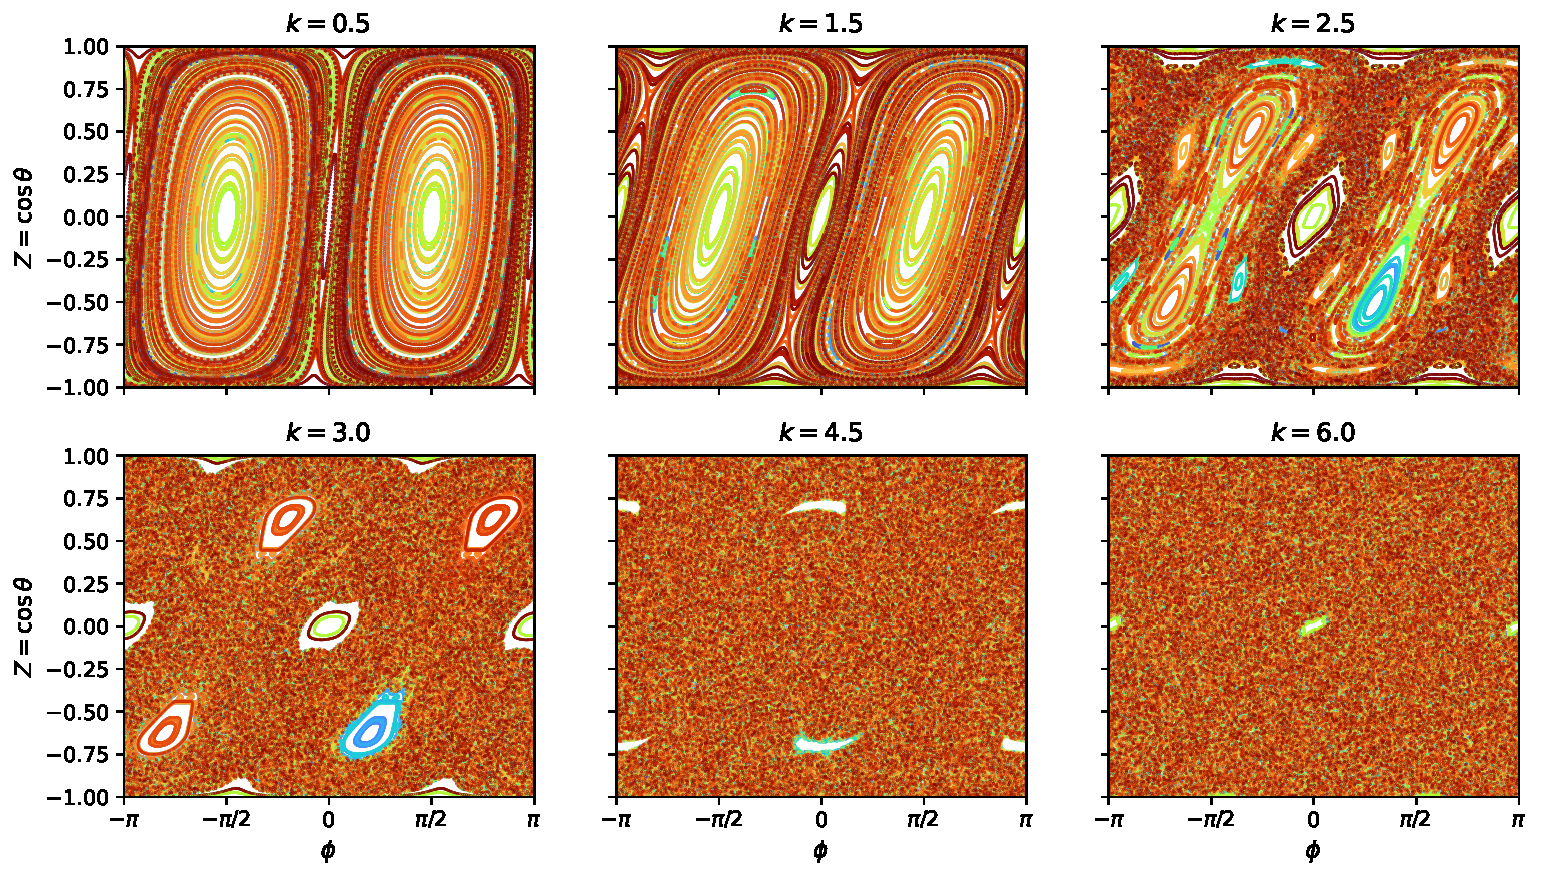
\includegraphics[width=\textwidth]{figures/portraits.pdf}
  \caption{Phase portraits of the kicked top for $p = \pi/2$ and increasing $k$, in the canonical coordinates
  $(\phi, Z=\cos\theta)$ (equal areas in the plot are equal areas on the sphere). Each panel shows a $20\times20$
  equal-area grid of initial conditions iterated for $500$ kicks, one colour per orbit. Closed curves are regular
  (quasi-periodic) orbits. Uniformly speckled regions are filled by chaotic orbits.}
  \label{fig:portraits}
\end{figure}

\subsection{Regular motion}

Along an invariant curve, parametrise the position by an angle $\vartheta$ that runs once around the curve. If
$\vartheta$ advances by $\vartheta_{n+1} - \vartheta_n$ per kick, the \emph{rotation number}
\begin{equation*}
  \nu = \lim_{n\to\infty}\frac{\vartheta_n - \vartheta_0}{2\pi n}
\end{equation*}
is the average fraction of a full turn per kick. If $\nu$ is irrational, the orbit fills the curve densely
(\emph{quasi-periodic} motion). If $\nu = r/q$ is rational, the orbit is periodic with period $q$. In a phase portrait,
regular orbits appear as smooth closed curves.

\paragraph{Why small $k$ looks integrable at $p = \pi/2$.} For small $k$ (\cref{fig:portraits}, $k=0.5$), the phase
portrait looks almost integrable, although the unperturbed map $R = R_y(\pi/2)$ is degenerate: $R^4 = R_y(2\pi) = I$,
every orbit has period 4. So look at four periods at once. Write $F = TR$, with $T$ the torsion, the time-$1$ flow of
the kick Hamiltonian $h_T = \frac k2 Z^2$ (Step 2 of \cref{sec:map}). Inserting $R^{-m}R^m = I$,
\begin{equation*}
  F^4 = TRTRTRTR = T\,\big(RTR^{-1}\big)\,\big(R^2TR^{-2}\big)\,\big(R^3TR^{-3}\big)\,R^4 ,
  \qquad R^4 = I .
\end{equation*}
Each factor $R^mTR^{-m}$ is again the time-$1$ flow of a Hamiltonian, namely $h_T\circ R^{-m}$ ($h_T$ evaluated at
$R^{-m}\vs$). To see this, let $\vs(t)$ follow $h_T$ and put $\bm u = R^m\vs$. Rotations preserve cross products, and by
the chain rule $\nabla_{\!u}\big[h_T(R^{-m}\bm u)\big] = R^m\,\nabla_{\!s}h_T$ (because $R^{-m} = (R^m)^{\mathsf T}$),
so
\begin{equation*}
  \dot{\bm u} = R^m\big(\nabla_{\!s}h_T\times\vs\big) = \big(R^m\nabla_{\!s}h_T\big)\times\big(R^m\vs\big)
  = \nabla_{\!u}\big[h_T\circ R^{-m}\big]\times\bm u .
\end{equation*}
From \eqref{eq:rotations}, the $z$ component of $R^{-m}\vs$ is $Z$, $X$, $-Z$, $-X$ for $m = 0, 1, 2, 3$, so the four
Hamiltonians are $\frac k2 Z^2$, $\frac k2X^2$, $\frac k2 Z^2$, $\frac k2X^2$. Each factor is the identity plus a
correction of order $k$, so to first order in $k$ the product is the time-$1$ flow of the sum,
\begin{equation}\label{eq:hbar}
  \bar h = \frac{k}{2}\,\big(Z^2 + X^2 + Z^2 + X^2\big) = k\,(X^2 + Z^2) = k\,(1 - Y^2).
\end{equation}
$\nabla_{\!s}\bar h = -2kY\,\hat{\bm y}$, so the flow of $\bar h$ is a rotation about $y$ with rate $-2kY$, and $Y$ is
conserved. The invariant curves of $F^4$ are therefore close to circles $Y = \sqrt{1-Z^2}\sin\phi = $ const around the
poles $\pm\hat{\bm y}$. In the $(\phi,Z)$ plane these are the closed curves around $(\pm\pi/2, 0)$ in the $k=0.5$
panel. On the great circle $Y = 0$ (the lines $\phi = 0, \pm\pi$) the rate $-2kY$ vanishes, so higher-order terms
decide what happens there. Numerically a thin chaotic layer forms along these lines.

\subsection{KAM theorem and the breakup of invariant curves}

What happens to invariant curves when an integrable map is perturbed? The answer is given by the
Kolmogorov--Arnold--Moser (KAM) theorem. Call a number $\nu$ \emph{sufficiently irrational} if it is badly
approximated by fractions: $|\nu - r/q| \ge C/q^{\tau}$ for all integers $r, q$, for some constants $C > 0$ and $\tau
\ge 2$. Stated informally:
\begin{theorem*}[KAM, informal]
For a sufficiently small smooth perturbation of an integrable area-preserving twist map, most invariant curves
survive, only slightly deformed. The survivors are those whose rotation number $\nu$ is sufficiently irrational. The
destroyed curves occupy a fraction of phase space that goes to zero with the perturbation.
\end{theorem*}
The curves with rational rotation number $\nu = r/q$ do not survive. By the Poincaré--Birkhoff theorem, such a curve
breaks up into a chain of alternating elliptic and hyperbolic period-$q$ points. Around the elliptic ones there are new
small islands. Each hyperbolic point has a \emph{stable manifold} (the curve of points that approach it under
repeated application of $F$) and an \emph{unstable manifold} (the points that approach it under $F^{-1}$). These two
curves intersect in an infinitely folded pattern (a \emph{homoclinic tangle}), which produces a thin chaotic layer.
The structure repeats on ever finer scales: islands around islands.

As $k$ grows, the chaotic layers widen. When neighbouring resonances (island chains) grow until they overlap
(Chirikov's resonance-overlap criterion), the KAM curves that separated them are destroyed and the layers merge into a
connected \emph{chaotic sea}. In a 2D map, surviving KAM curves are impenetrable barriers: a chaotic orbit can never
enter an island and a regular orbit can never leave one.

\subsection{Mixed and global chaos in the kicked top}

\Cref{fig:portraits} shows the scenario for $p = \pi/2$:
\begin{itemize}
  \item $k = 0.5$ and $1.5$: almost everything is regular. Large families of closed curves surround the stable poles
  $\pm\hat{\bm y}$ ($|\Tr M_\pm| = k < 2$, \eqref{eq:pole-trace}), with thin chaotic layers near $\phi = 0, \pm\pi$.
  \item $k = 2.5$: the poles have just become unstable (\cref{sec:poles}). Chaos spreads from them, and the new
  islands of $\vs_\pm$ and of the period-2 orbit appear, together with a mixture of smaller island chains.
  \item $k = 3$: a \emph{mixed phase space}. A large chaotic sea surrounds islands around $\vs_\pm$ (at $(0.63,
  -0.63)$ and its mirror image $(2.51, 0.63)$), around the period-2 orbit (at $(-0.63, 0.63)$ and $(-2.51, -0.63)$),
  and around the period-4 orbit (at $(0,0)$, $(\pm\pi, 0)$ and near $Z = \pm1$). The pairing of islands under $S$
  of \eqref{eq:symmetry} is clearly visible.
  \item $k = 4.5$ and $6$: almost \emph{global chaos}. The islands of $\vs_\pm$ are gone ($k > \pi\sqrt2$) and only
  tiny islands remain (e.g.\ the period-4 island at $(0,0)$ for $k=6$, where $|\Tr M^{(4)}| < 2$ by
  \eqref{eq:period4-trace}).
\end{itemize}

\Cref{fig:single-orbits} shows the difference between the two kinds of motion for $k=3$. A single orbit started
inside the island around $\vs_+$ stays on a closed curve. A single orbit started next to the unstable pole
$+\hat{\bm y}$ wanders through the whole chaotic sea but never enters any island. \Cref{fig:sphere} shows the $k=3$
portrait on the sphere itself.

\begin{figure}[!htbp]
  \centering
  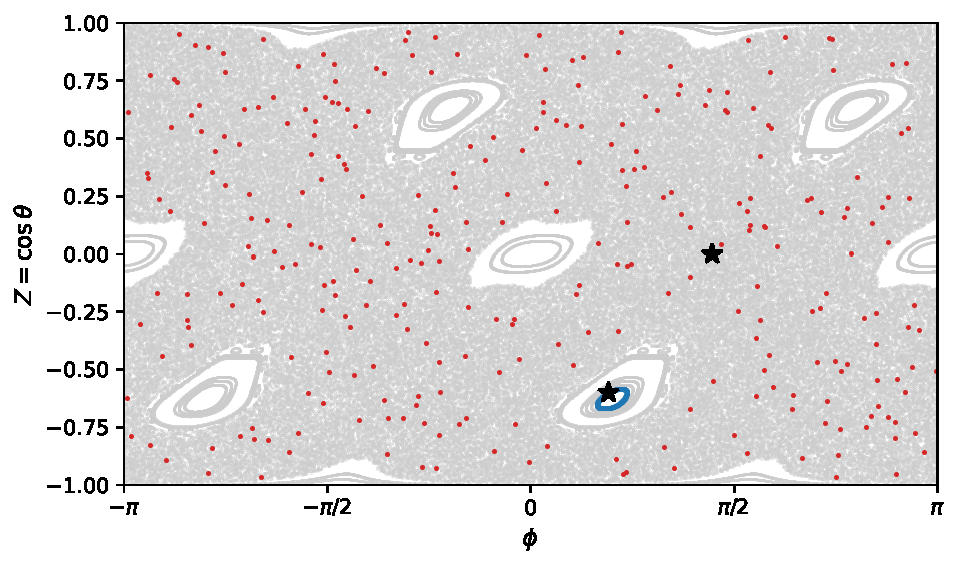
\includegraphics[width=0.75\textwidth]{figures/single_orbits.pdf}
  \caption{Two single orbits for $p = \pi/2$, $k = 3$, $300$ kicks each, on top of the full portrait (grey). Blue:
  started at $(\phi_0, Z_0) = (0.6, -0.6)$, inside the island of $\vs_+$. Red: started at $(1.4, 0)$, near the
  hyperbolic pole $+\hat{\bm y}$. Stars mark the starting points.}
  \label{fig:single-orbits}
\end{figure}

\begin{figure}[!htbp]
  \centering
  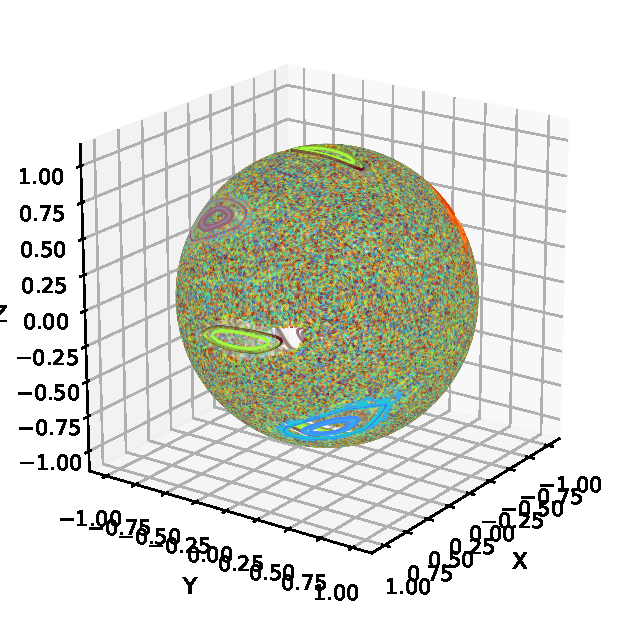
\includegraphics[width=0.5\textwidth]{figures/sphere.pdf}
  \caption{The $k=3$ phase portrait of \cref{fig:portraits} drawn on the unit sphere $(X,Y,Z)$.}
  \label{fig:sphere}
\end{figure}

%---------------------------------------------------------------------
\section{Lyapunov exponents}\label{sec:lyapunov}

Chaos means \emph{sensitive dependence on initial conditions}. Two orbits starting a small distance $d_0$ apart
separate exponentially, $d_n \sim d_0\, e^{\Lambda n}$. The rate $\Lambda$ is the (maximal) \emph{Lyapunov exponent}.

\paragraph{Definition.} Let $\vs_0, \vs_1, \dots$ be an orbit and $\delta\vs_0$ a small displacement of its starting
point. By the linearisation of \cref{sec:stability}, $\delta\vs_1 = DF(\vs_0)\,\delta\vs_0$, $\delta\vs_2 =
DF(\vs_1)\,\delta\vs_1$, and so on, so $\delta\vs_n = M_n\,\delta\vs_0$ with the \emph{tangent map}
\begin{equation*}
  M_n = DF(\vs_{n-1})\cdots DF(\vs_1)\,DF(\vs_0).
\end{equation*}
With $\|\bm v\|$ the length of a vector,
\begin{equation}\label{eq:lyapunov}
  \Lambda = \lim_{n\to\infty} \frac{1}{n}\ln\frac{\|M_n\,\delta\vs_0\|}{\|\delta\vs_0\|} ,
\end{equation}
which for almost every $\delta\vs_0$ does not depend on the direction of $\delta\vs_0$. For an area-preserving 2D map
$\det M_n = 1$: stretching by $e^{\Lambda n}$ in one direction is compensated by shrinking by $e^{-\Lambda n}$ in
another, so the two exponents are $\pm\Lambda$. Typical values:
\begin{itemize}
  \item regular (quasi-periodic) orbits: $\Lambda = 0$. Nearby orbits on neighbouring invariant curves separate only
  linearly, $d_n \propto n$, because their rotation numbers differ slightly, and $\frac1n\ln n \to 0$;
  \item a hyperbolic fixed point with eigenvalue $\lambda_u$: there $M_n = M^n$, so $\|M_n\delta\vs_0\| \sim
  |\lambda_u|^n$ and $\Lambda = \ln|\lambda_u|$. For the pole $+\hat{\bm y}$ at $k=3$, \eqref{eq:pole-trace} gives
  $\Tr M = 3$, so $\lambda^2 - 3\lambda + 1 = 0$, $\lambda_u = (3+\sqrt5)/2 \approx 2.62$ and $\Lambda \approx 0.96$;
  \item chaotic orbits: $\Lambda > 0$. The value is an average over the whole chaotic sea, which contains regions of
  very different local stretching.
\end{itemize}

\Cref{fig:divergence} shows this directly. Pairs of orbits are started with $\theta_0$ differing by $10^{-8}$. In the
island the distance stays at $\sim10^{-8}$. In the chaotic sea it grows exponentially until it saturates at the size of
the sphere (at most $2$, the diameter). Taking the logarithm of $d_n \sim d_0e^{\Lambda n}$ gives $\ln d_n \approx \ln
d_0 + \Lambda n$, a straight line of slope $\Lambda$. A straight-line fit of $\ln d_n$ for $5 \le n \le 40$ gives a
slope of about $0.47$ per kick. This is a rough, finite-time estimate from a single pair. A reliable value of $\Lambda$
needs \eqref{eq:lyapunov} evaluated over long times, with $\delta\vs$ rescaled to unit length every few kicks so that it
never leaves the linear regime (the method of Benettin \emph{et al.}~\cite{Benettin}). The code computes $\Lambda$
in exactly this way (\cref{sec:benettin}).

\begin{figure}[!htbp]
  \centering
  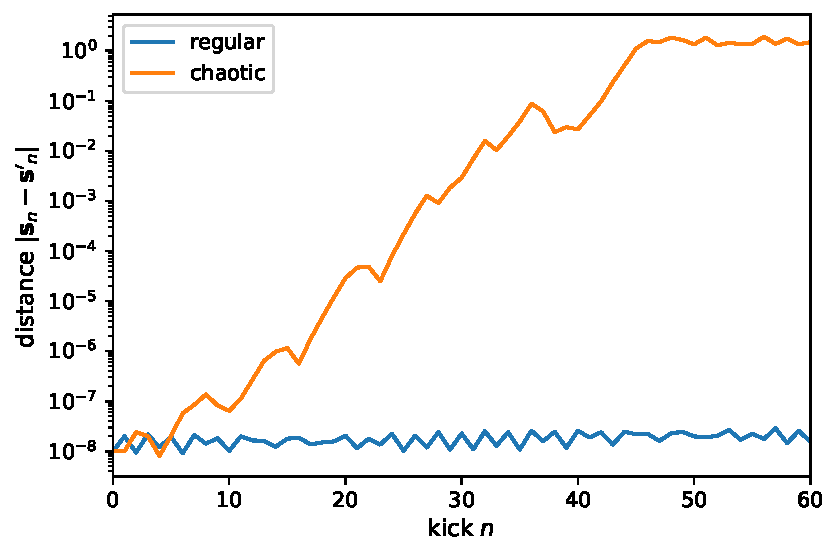
\includegraphics[width=0.6\textwidth]{figures/divergence.pdf}
  \caption{Distance between two orbits whose initial $\theta_0$ differ by $10^{-8}$, for $p = \pi/2$, $k = 3$. Blue:
  both inside the island of $\vs_+$. Orange: both in the chaotic sea. The straight segment on the logarithmic axis is
  exponential separation.}
  \label{fig:divergence}
\end{figure}

\subsection{Computing \texorpdfstring{$\Lambda$}{Lambda}: the tangent map and the Benettin algorithm}\label{sec:benettin}

\paragraph{The tangent map for any $p$.} The definition \eqref{eq:lyapunov} needs $DF(\vs)\,\delta\vs$, the image of a
small displacement under one kick. Write the map \eqref{eq:map} as $F(\vs) = R_z\big(kZ'(\vs)\big)\,\vs'(\vs)$ with
$\vs' = R_y(p)\,\vs$ and $Z' = (\vs')_z$, and vary $\vs \to \vs + \delta\vs$.
\begin{enumerate}
  \item The rotation is linear: $\delta\vs' = R_y(p)\,\delta\vs$, and $\delta Z' = (\delta\vs')_z$.
  \item The torsion depends on $\vs'$ twice, through the vector it rotates and through its angle $kZ'$. By the
  product rule,
  \[ \delta\big[R_z(kZ')\,\vs'\big] = R_z(kZ')\,\delta\vs' + \frac{dR_z}{d\alpha}\Big|_{\alpha = kZ'}\vs'\;k\,\delta Z' . \]
  \item With $\frac{d}{d\alpha}R_z(\alpha)\bm v = \hat{\bm z}\times R_z(\alpha)\bm v$ (\cref{sec:precession}) and
  $R_z(kZ')\vs' = \vs_{n+1}$, the last term is $k\,\delta Z'\,\hat{\bm z}\times\vs_{n+1}$.
\end{enumerate}
Hence
\begin{equation}\label{eq:tangent}
  \boxed{\delta\vs_{n+1} = DF(\vs_n)\,\delta\vs_n = R_z(kZ')\,\delta\vs' + k\,\delta Z'\;\hat{\bm z}\times\vs_{n+1},
  \qquad \delta\vs' = R_y(p)\,\delta\vs_n .}
\end{equation}
(For $p = \pi/2$ and the points of the period-4 orbit this reduces to the $DT$ used in \cref{sec:pi2}.) The image is
again tangent to the sphere. If $\vs_n\cdot\delta\vs_n = 0$, then, because rotations preserve dot products and $\hat{\bm
z}\times\vs_{n+1}$ is perpendicular to $\vs_{n+1}$,
\begin{equation*}
  \vs_{n+1}\cdot\delta\vs_{n+1} = \big(R_z\vs'\big)\cdot\big(R_z\delta\vs'\big) = \vs'\cdot\delta\vs' = \vs_n\cdot\delta\vs_n = 0 .
\end{equation*}

\paragraph{The algorithm.} $\delta\vs_n = M_n\delta\vs_0$ grows like $e^{\Lambda n}$, and for $\Lambda \approx 0.4$ it
overflows double precision ($\approx 10^{308}$) after about $\ln(10^{308})/0.4 \approx 1800$ kicks. Since
\eqref{eq:tangent} is linear in $\delta\vs$, the vector can be rescaled at any time without changing its direction.
Benettin's algorithm does exactly this:
\begin{enumerate}
  \item start from a unit tangent vector $\delta\vs_0$, $\vs_0\cdot\delta\vs_0 = 0$;
  \item apply \eqref{eq:tangent} and \eqref{eq:map} together, kick by kick;
  \item every $m$ kicks, measure the length $d_j = \|\delta\vs\|$ and rescale, $\delta\vs \to \delta\vs/d_j$;
  \item after $N$ kicks, $\Lambda_N = \frac1N\sum_j \ln d_j$.
\end{enumerate}
Because every rescaling only divides by the length just measured, $\prod_j d_j = \|M_N\,\delta\vs_0\|$, so $\Lambda_N$
is exactly \eqref{eq:lyapunov} evaluated at the finite time $N$, without overflow. $\Lambda_N$ converges to $\Lambda$ as
$N\to\infty$. At finite $N$ there are two kinds of error. The first part of the evolution, before $\delta\vs$ has turned
into the most unstable direction, contributes a term of order $1/N$. On regular orbits $\|\delta\vs\|$ grows like $n$,
so $\Lambda_N \approx \ln N/N$, small but not zero.

\paragraph{Result for $k = 3$.} \Cref{fig:lyapunov-map} shows $\Lambda_N$ ($N = 2000$) for an $80\times80$ grid of
initial conditions. The islands of \cref{fig:portraits} appear as regions with $\Lambda_N \approx 0$, and the chaotic
sea has a nearly uniform value $\Lambda \approx 0.33$, as it must, since a single chaotic orbit visits the whole sea.
(The larger slope $\approx 0.47$ of \cref{fig:divergence} is a local rate over the first $40$ kicks near the
pole $+\hat{\bm y}$, where the stretching $\ln\lambda_u \approx 0.96$ is stronger than the average.)

\begin{figure}[!htbp]
  \centering
  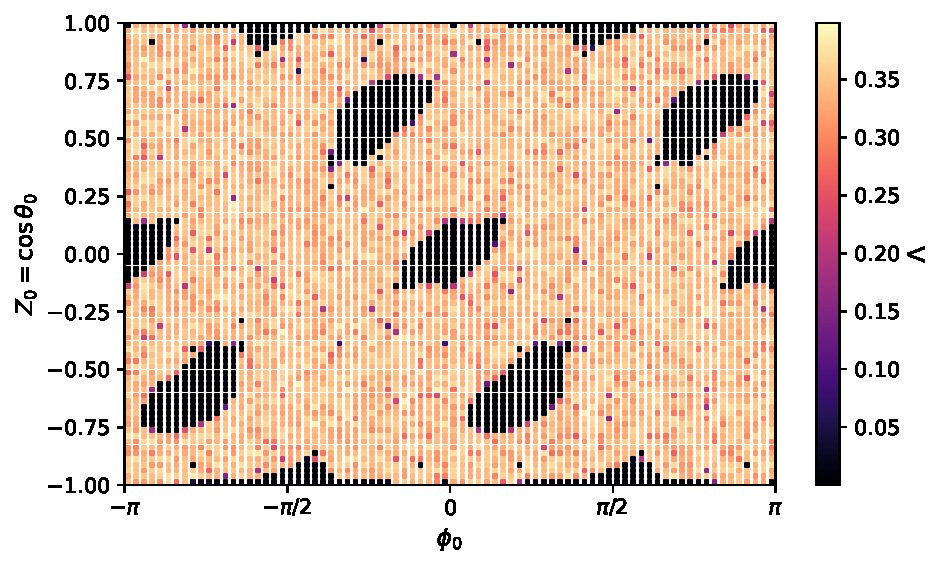
\includegraphics[width=0.75\textwidth]{figures/lyapunov_map.pdf}
  \caption{Finite-time Lyapunov exponent $\Lambda_N$ ($N = 2000$ kicks, Benettin algorithm with rescaling every kick)
  of each initial condition of an $80\times80$ equal-area grid, $p = \pi/2$, $k = 3$. Dark: regular islands
  ($\Lambda_N\approx0$). Bright: chaotic sea ($\Lambda\approx0.33$).}
  \label{fig:lyapunov-map}
\end{figure}

%---------------------------------------------------------------------
%=====================================================================
\part{The quantum kicked top}\label{part:quantum}
%=====================================================================

\section{Quantum spin}\label{sec:quantum}

In quantum mechanics the three components of the angular momentum become Hermitian operators $\hat J_x, \hat J_y,
\hat J_z$ (in this part a hat marks an operator, except on bold unit vectors). We use units with $\hbar = 1$. The
classical bracket \eqref{eq:J-algebra} is replaced by the commutator $[\hat A, \hat B] = \hat A\hat B - \hat B\hat A$
with the rule $\PB{\cdot}{\cdot} \to -i[\cdot,\cdot]$:
\begin{equation}\label{eq:q-algebra}
  [\hat J_a, \hat J_b] = i\,\epsilon_{abc}\,\hat J_c .
\end{equation}

\paragraph{The basis $|j,m\rangle$.} $\hat J^2 = \hat J_x^2 + \hat J_y^2 + \hat J_z^2$ commutes with every $\hat J_a$
(the quantum version of the Casimir of \cref{sec:angmom}), so $\hat J^2$ and $\hat J_z$ have common eigenvectors.
The standard result of the angular-momentum algebra is
\begin{equation}\label{eq:jm-basis}
  \hat J^2|j,m\rangle = j(j+1)\,|j,m\rangle, \qquad \hat J_z|j,m\rangle = m\,|j,m\rangle, \qquad
  m = j, j-1, \dots, -j,
\end{equation}
where $j$ is a fixed integer or half-integer. The space of states is therefore $(2j+1)$-dimensional, and a state is a
column vector $|\psi\rangle = \sum_m \psi_m|j,m\rangle$ of $2j+1$ complex numbers $\psi_m$ with $\sum_m|\psi_m|^2 = 1$.

\paragraph{Ladder operators.} $\hat J_\pm = \hat J_x \pm i\hat J_y$ raise and lower $m$ by one:
\begin{equation}\label{eq:ladder}
  \hat J_+|j,m\rangle = a(m)\,|j,m+1\rangle, \qquad \hat J_-|j,m+1\rangle = a(m)\,|j,m\rangle, \qquad
  a(m) = \sqrt{j(j+1) - m(m+1)} .
\end{equation}
(Derivation of $a(m)$: $\hat J_-\hat J_+ = \hat J^2 - \hat J_z^2 - \hat J_z$ by \eqref{eq:q-algebra}, so
$\|\hat J_+|j,m\rangle\|^2 = \langle j,m|\hat J_-\hat J_+|j,m\rangle = j(j+1) - m^2 - m$.) Hence $\hat J_y = (\hat J_+ -
\hat J_-)/(2i)$ has the only non-zero matrix elements
\begin{equation}\label{eq:jy-elements}
  \langle j,m+1|\hat J_y|j,m\rangle = -\frac{i}{2}\,a(m), \qquad \langle j,m|\hat J_y|j,m+1\rangle = +\frac{i}{2}\,a(m),
\end{equation}
and $\langle\hat J_+\rangle = \langle\hat J_x\rangle + i\langle\hat J_y\rangle = \sum_m \psi_{m+1}^*\,a(m)\,\psi_m$
gives the two transverse expectation values ($^*$ is complex conjugation).

\section{The Floquet operator}\label{sec:floquet}

\paragraph{Derivation.} The state obeys the Schrödinger equation $i\,\frac{d}{dt}|\psi\rangle = \hat H(t)|\psi\rangle$
with $\hat H(t)$ the operator version of \eqref{eq:H}. We integrate it over one period exactly as in \cref{sec:map}.
\begin{enumerate}
  \item For $n < t < n+1$, $\hat H = p\hat J_y$ does not depend on time, so $|\psi(t)\rangle = e^{-i(t-n)p\hat
  J_y}|\psi(n^+)\rangle$. After the unit time, $|\psi\rangle \to \hat R\,|\psi\rangle$ with $\hat R = e^{-ip\hat J_y}$.
  \item Across the kick only the $\delta$ term matters (the same argument as Step 2 of \cref{sec:map}):
  $i\frac{d}{dt}|\psi\rangle = \frac{k}{2j}\hat J_z^2\,\delta(t-n-1)|\psi\rangle$. All operators involved commute
  with each other, so the solution is the exponential of the integral,
  $|\psi\rangle \to \hat K|\psi\rangle$ with $\hat K = e^{-i\frac{k}{2j}\hat J_z^2}$.
\end{enumerate}
One period is therefore
\begin{equation}\label{eq:floquet}
  \boxed{\hat U = \hat K\hat R = \exp\!\Big(-i\frac{k}{2j}\hat J_z^2\Big)\exp\!\big(-ip\hat J_y\big), \qquad
  |\psi_{n+1}\rangle = \hat U|\psi_n\rangle ,}
\end{equation}
first the rotation, then the kick, as in \eqref{eq:map}. In the basis \eqref{eq:jm-basis} the kick is diagonal,
$\hat K|j,m\rangle = e^{-ikm^2/(2j)}|j,m\rangle$. $\hat U$ is unitary ($\hat U^\dagger\hat U = 1$, $^\dagger$ the conjugate
transpose) because it is a product of exponentials of $-i$ times Hermitian operators; hence $\langle\psi_n|\psi_n\rangle$
is conserved.

\paragraph{The rotation in matrix form.} $\hat J_y$ is Hermitian, so it has an orthonormal basis of eigenvectors,
$\hat J_y = \hat V\,\mathrm{diag}(\mu_l)\,\hat V^\dagger$ with eigenvalues $\mu_l = -j, -j+1, \dots, j$ (the same
spectrum as $\hat J_z$, since $\hat J_y$ is $\hat J_z$ rotated). Then
\begin{equation}\label{eq:exp-jy}
  e^{-i\alpha\hat J_y} = \hat V\,\mathrm{diag}\big(e^{-i\alpha\mu_l}\big)\,\hat V^\dagger
\end{equation}
for any angle $\alpha$, because $(\hat V D\hat V^\dagger)^n = \hat V D^n\hat V^\dagger$ term by term in the exponential
series.

\paragraph{The classical limit.} Write $\hat{\bm s} = \hat{\vJ}/j$. Then \eqref{eq:q-algebra} becomes $[\hat s_a, \hat
s_b] = \frac{i}{j}\,\epsilon_{abc}\,\hat s_c$: the components of $\hat{\bm s}$ commute in the limit $j\to\infty$, and
$1/j$ plays the role of an effective Planck constant. In the Heisenberg picture an operator evolves as $\hat A \to
\hat U^\dagger\hat A\hat U$. For the rotation, $\hat R^\dagger\hat J_a\hat R = \sum_b R_y(p)_{ab}\hat J_b$ (the quantum
rotation rotates the vector operator exactly as \eqref{eq:rotation-y}). For the kick, $\hat J_z$ commutes with $\hat K$,
and for $\hat J_+$, using $\hat J_+ f(\hat J_z) = f(\hat J_z - 1)\hat J_+$,
\begin{equation*}
  \hat K^\dagger\hat J_+\hat K = e^{i\frac{k}{2j}\hat J_z^2}\,e^{-i\frac{k}{2j}(\hat J_z-1)^2}\,\hat J_+
  = e^{i\frac{k}{2j}(2\hat J_z - 1)}\,\hat J_+ = e^{ik\hat s_z - \frac{ik}{2j}}\,\hat J_+ ,
\end{equation*}
i.e.\ $\hat J_x + i\hat J_y$ is rotated about $z$ by the angle $k\hat s_z - k/(2j)$. For $j\to\infty$ this is the
torsion \eqref{eq:torsion} with angle $kZ$. So the Heisenberg equations of $\hat{\bm s}$ reduce to the classical map
\eqref{eq:map} when $j\to\infty$.

\section{Spin coherent states and the Husimi distribution}\label{sec:coherent}

\paragraph{Coherent states.} The state $|j,j\rangle$ points along $+\hat{\bm z}$ as sharply as quantum mechanics
allows: $\langle\hat{\vJ}\rangle = (0,0,j)$. Rotating it to the direction $\bm n(\theta,\phi)$ of \eqref{eq:unit}
gives the spin coherent state
\begin{equation}\label{eq:coherent}
  |\theta,\phi\rangle = e^{-i\phi\hat J_z}\,e^{-i\theta\hat J_y}\,|j,j\rangle
  = \sum_m \sqrt{\binom{2j}{j-m}}\;\cos^{j+m}\!\tfrac{\theta}{2}\;\sin^{j-m}\!\tfrac{\theta}{2}\;e^{-im\phi}\;|j,m\rangle .
\end{equation}
The coefficients follow from writing the spin $j$ as $2j$ spins $\frac12$ all pointing along $\bm n$: each spin
$\frac12$ is $\cos\frac\theta2|\!\uparrow\rangle + \sin\frac\theta2\,e^{i\phi}|\!\downarrow\rangle$ up to a phase, and
$|j,m\rangle$ is the normalised symmetric combination of $j+m$ up and $j-m$ down spins; collecting the
$\binom{2j}{j-m}$ terms gives \eqref{eq:coherent} (the overall phase $e^{-ij\phi}$ is dropped). Three properties:
\begin{enumerate}
  \item Normalisation: $\sum_m\binom{2j}{j-m}\cos^{2(j+m)}\frac\theta2\sin^{2(j-m)}\frac\theta2 =
  (\cos^2\frac\theta2 + \sin^2\frac\theta2)^{2j} = 1$ by the binomial theorem.
  \item $\langle\theta,\phi|\hat{\vJ}|\theta,\phi\rangle = j\,\bm n(\theta,\phi)$, because the rotations carry
  $\langle\hat{\vJ}\rangle = j\hat{\bm z}$ to $j\bm n$.
  \item Width: in $|j,j\rangle$, $\langle\hat J_x^2\rangle = \langle\hat J_y^2\rangle = \frac12(j(j+1) - j^2) =
  \frac j2$. So the uncertainty of $\hat{\bm s}$ transverse to $\bm n$ is $\sqrt{1/(2j)}$ per direction: a coherent
  state is a blob of radius $\sim 1/\sqrt j$ on the unit sphere, and the spread
  $(\langle\hat J^2\rangle - |\langle\hat{\vJ}\rangle|^2)/j^2 = (j(j+1)-j^2)/j^2 = 1/j$.
\end{enumerate}
The overlap of two coherent states is $|\langle\bm n|\bm n'\rangle|^2 = \big(\frac{1+\bm n\cdot\bm n'}{2}\big)^{2j}$
(for $\bm n = \hat{\bm z}$ it is $\cos^{4j}\frac{\theta'}{2}$ from \eqref{eq:coherent}; rotations give the general case).

\paragraph{Husimi distribution.} The Husimi function of a state $|\psi\rangle$ is
\begin{equation}\label{eq:husimi}
  Q(\theta,\phi) = |\langle\theta,\phi|\psi\rangle|^2
  = \Big|\sum_m \sqrt{\tbinom{2j}{j-m}}\cos^{j+m}\!\tfrac{\theta}{2}\sin^{j-m}\!\tfrac{\theta}{2}\,e^{im\phi}\,\psi_m\Big|^2 ,
\end{equation}
the probability that $|\psi\rangle$ is found in the coherent state at $(\theta,\phi)$. $0 \le Q \le 1$, and $Q$ is the
quantum analogue of a density on the classical phase space: plotted in the canonical coordinates $(\phi, Z)$ it can be
compared directly with the phase portraits of \cref{sec:chaos}. Its normalisation follows from the resolution of the
identity
\begin{equation}\label{eq:resolution}
  \frac{2j+1}{4\pi}\int |\theta,\phi\rangle\langle\theta,\phi|\,d\Omega = \hat 1, \qquad d\Omega = d\phi\,dZ ,
\end{equation}
which holds because the left side commutes with all rotations (so it is a multiple of $\hat1$ by Schur's lemma) and its
trace is $\frac{2j+1}{4\pi}\int d\Omega = 2j+1$. Taking $\langle\psi|\cdot|\psi\rangle$ of \eqref{eq:resolution},
\begin{equation}\label{eq:husimi-norm}
  \frac{2j+1}{4\pi}\int Q\,d\Omega = 1 .
\end{equation}
For a coherent state centred at $\bm n_0$, $Q = \big(\frac{1+\bm n\cdot\bm n_0}{2}\big)^{2j} \approx e^{-j\,|\bm n -
\bm n_0|^2/2}$: a Gaussian of width $1/\sqrt j$.

\paragraph{Quantum--classical correspondence and the Ehrenfest time.} Start from a coherent state at $\bm n_0$. As long
as its blob of size $1/\sqrt j$ stays small, each part of it follows the classical map, so $\langle\hat{\bm s}\rangle_n$
follows the classical orbit $\bm s_n$ from $\bm n_0$. In a regular island nearby orbits separate only linearly and the
agreement lasts long. In the chaotic sea the blob is stretched as $e^{\Lambda n}$ (\cref{sec:lyapunov}); it covers a
region of size one when $j^{-1/2}e^{\Lambda n} \sim 1$, i.e.\ after
\begin{equation}\label{eq:ehrenfest}
  n_E \simeq \frac{\ln j}{2\Lambda}
\end{equation}
kicks (the Ehrenfest time). After $n_E$, $\langle\hat{\bm s}\rangle$ no longer follows any single orbit and the spread
grows to order one.

\section{Symmetry and quasienergy spectrum}\label{sec:qspectrum}

\paragraph{Parity.} Let $\hat P = e^{-i\pi\hat J_y}$, the quantum version of $S = R_y(\pi)$ of \eqref{eq:symmetry}.
$\hat P$ commutes with $\hat R = e^{-ip\hat J_y}$ (both are functions of $\hat J_y$). It also commutes with $\hat K$: $\hat
P^\dagger\hat J_z\hat P = -\hat J_z$ (rotation by $\pi$ about $y$ reverses $z$), so $\hat P^\dagger\hat J_z^2\hat P = \hat
J_z^2$ and $\hat P^\dagger\hat K\hat P = \hat K$. Hence $[\hat U, \hat P] = 0$. By \eqref{eq:exp-jy} the eigenvalues of
$\hat P$ are $e^{-i\pi\mu_l}$; consecutive $\mu_l$ differ by one, so $e^{-i\pi\mu_l}$ alternates in sign along $l$. The
eigenvectors of $\hat J_y$ with odd $l$ span one parity sector, those with even $l$ the other, and $\hat U$ is
block-diagonal in this basis.

\paragraph{Quasienergies.} $\hat U$ is unitary, so its eigenvalues lie on the unit circle:
$\hat U|\varepsilon\rangle = e^{-i\varepsilon}|\varepsilon\rangle$ with quasienergy $\varepsilon \in [-\pi, \pi)$
(defined modulo $2\pi$, like a phase). In each sector of $N_s$ levels the mean spacing is $2\pi/N_s$ and the density is
uniform on the circle, so the spacings are unfolded simply as
\begin{equation}\label{eq:unfold}
  s_i = \frac{N_s}{2\pi}\,(\varepsilon_{i+1} - \varepsilon_i), \qquad \langle s\rangle = 1 ,
\end{equation}
with the last spacing wrapping around the circle.

\paragraph{Spacing statistics.} The distribution $P(s)$ of the $s_i$ within one sector is a standard fingerprint of
chaos. For regular dynamics levels are typically uncorrelated and $P(s) = e^{-s}$ (Poisson). For chaotic dynamics
levels repel and $P(s)$ follows random-matrix theory. With an antiunitary (generalised time-reversal) symmetry, which
the kicked top has, the relevant ensemble is the circular orthogonal ensemble (COE), well approximated by the Wigner
surmise; without it, the circular unitary ensemble (CUE):
\begin{equation}\label{eq:wigner}
  P_{\mathrm{P}}(s) = e^{-s}, \qquad P_{\mathrm{COE}}(s) = \frac{\pi s}{2}\,e^{-\pi s^2/4}, \qquad
  P_{\mathrm{CUE}}(s) = \frac{32 s^2}{\pi^2}\,e^{-4s^2/\pi} .
\end{equation}
A second measure needs no unfolding: the ratio of neighbouring spacings
\begin{equation}\label{eq:gap-ratio}
  r_i = \frac{\min(s_i, s_{i+1})}{\max(s_i, s_{i+1})} .
\end{equation}
Its mean is $\langle r\rangle = 2\ln2 - 1 \approx 0.386$ for Poisson, $\approx 0.531$ for the COE and $\approx 0.600$
for the CUE \cite{Atas2013}. Levels of different sectors do not repel, so mixing two sectors spoils both measures;
that is why the sectors are treated separately.

\paragraph{The special value $p = \pi/2$.} At $p = \pi/2$ the code finds $\langle r\rangle \approx 0.54$ in one parity
sector but only $\approx 0.41$--$0.44$ in the other, even for strongly chaotic $k$ and $j = 1000$. A value near
$0.42$ is what a superposition of two independent COE spectra gives, which indicates an additional symmetry of
$\hat U$ at $p = \pi/2$ that splits that sector again. We have not identified it (the rotations by $\pi$ about $x$ and
$z$ and by $\pi/2$ about $z$ do not commute with $\hat U$). For spectral statistics we therefore use a generic value,
$p = 1.7$, where both sectors agree with the COE (\cref{sec:qcode}).

\paragraph{Experiments.} The kicked top was introduced by Haake, Ku\'s and Scharf \cite{HKS1987} as a model of quantum
chaos; Haake's book \cite{Haake} is the standard reference. It has been realised with the hyperfine spin of cesium
atoms \cite{Chaudhury2009} and with superconducting qubits \cite{Neill2016}.


%=====================================================================
\part{Numerics and code}\label{part:numerics}
%=====================================================================

\section{Numerical method}\label{sec:method}

\paragraph{Exact map, no integrator.} The equations of motion \eqref{eq:eom-s} are solved exactly over one period
(\cref{sec:map}), so the code never integrates a differential equation. It applies the closed-form map
\eqref{eq:map}: two rotations per kick, 4 trigonometric evaluations and a few multiplications. There is no time-step
error, and the only error is floating-point round-off. Since both steps are exact rotations, the norm $|\vs| = 1$
and the area preservation of \cref{sec:area} hold up to round-off. In practice $\big||\vs_n|-1\big| \lesssim
3\times10^{-15}$ after 500 kicks.

\paragraph{Round-off on chaotic orbits.} On a chaotic orbit any error, including a round-off error of $10^{-16}$,
grows like $e^{\Lambda n}$. With $\Lambda \approx 0.5$ a computed chaotic trajectory differs from the exact trajectory
with the same initial condition after roughly $\ln(10^{16})/0.5 \approx 70$ kicks. This does not make the
phase portraits wrong. The computed orbit is still an orbit of the map to round-off accuracy at every step, and (by
shadowing arguments) it stays close to some true orbit, so it explores the same chaotic sea. Individual chaotic
trajectories beyond that time should be read statistically, not pointwise.

\paragraph{Initial conditions.} Three modes are available.
\begin{itemize}
  \item \texttt{single}: one point given by $(\theta_0, \phi_0)$ through \eqref{eq:unit}.
  \item \texttt{grid}: an $n_\theta \times n_\phi$ grid of cell centres, uniform in $Z = \cos\theta \in [-1,1]$ and
  in $\phi \in [-\pi, \pi]$. By \eqref{eq:area} every grid cell has the same phase-space area, so the grid samples all
  regions of phase space with equal weight. A grid uniform in $\theta$ would oversample the poles.
  \item \texttt{random}: points with $Z$ and $\phi$ uniformly distributed, which by \eqref{eq:area} is the uniform
  distribution on the sphere.
\end{itemize}

\paragraph{Recording.} After \texttt{n\_transient} discarded kicks, the state is stored at kicks $n = 0, m, 2m,
\dots \le$ \texttt{n\_kicks}, where $m$ = \texttt{save\_every}. The initial point is stored as $n=0$ and
the map is applied once per kick, so stored points are always ``just after a kick'', as in \cref{sec:map}.

\paragraph{Parallelisation.} Different initial conditions are independent, so the loop over them is parallelised with
OpenMP. The default configuration ($20\times20$ grid, $500$ kicks) runs in under a second.

\section{Code structure}\label{sec:code}

The physics is in Fortran (\texttt{src/}); the Fortran code writes plot-ready files, and Python only reads and plots
them. \Cref{fig:flow} shows the data flow and \cref{tab:modules} maps each module to the equations it implements. In
the source, the header comment of every module and function cites the equations it implements by number and by
\LaTeX{} label, e.g.\ \texttt{! ... eq.~(20) [eq:map]}, so the reference can be found again with \texttt{grep} if the
numbering of these notes changes.

\begin{figure}[!htbp]
  \centering
  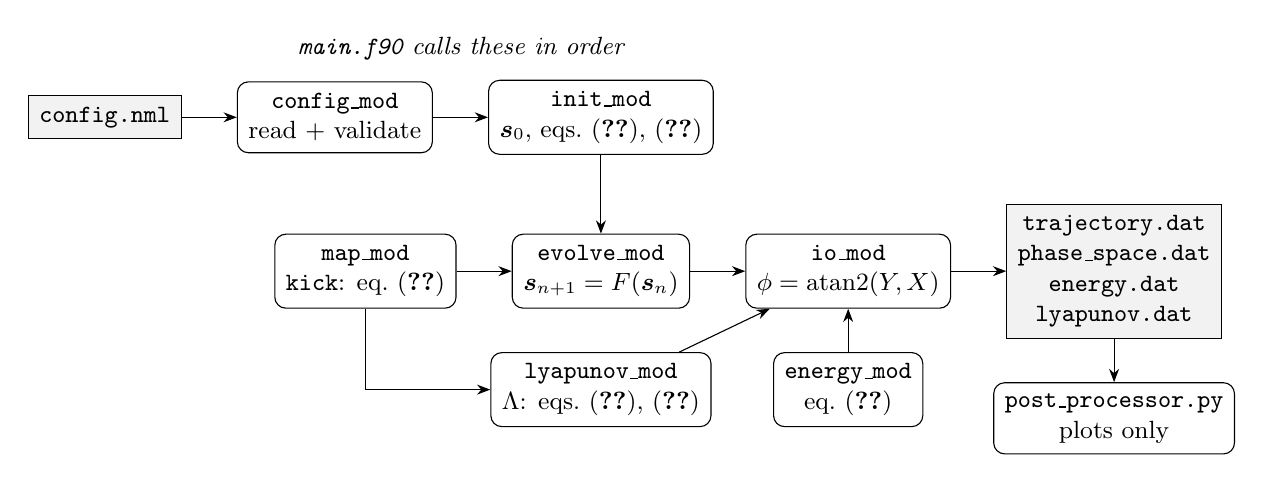
\begin{tikzpicture}[>=Stealth, node distance=0.55cm and 0.7cm,
      box/.style={draw, rounded corners, align=center, font=\small, minimum height=0.9cm, inner sep=4pt},
      file/.style={draw, shape=rectangle, fill=gray!10, align=center, font=\small\ttfamily, inner sep=4pt}]
    \node[file] (nml) {config.nml};
    \node[box, right=of nml] (cfg) {\texttt{config\_mod}\\ read + validate};
    \node[box, right=of cfg] (init) {\texttt{init\_mod}\\ $\vs_0$, eqs.~\eqref{eq:unit}, \eqref{eq:area}};
    \node[box, below=1.0cm of init] (evo) {\texttt{evolve\_mod}\\ $\vs_{n+1} = F(\vs_n)$};
    \node[box, left=of evo] (map) {\texttt{map\_mod}\\ \texttt{kick}: eq.~\eqref{eq:map}};
    \node[box, right=of evo] (io) {\texttt{io\_mod}\\ $\phi = \operatorname{atan2}(Y,X)$};
    \node[box, below=of io] (en) {\texttt{energy\_mod}\\ eq.~\eqref{eq:energy}};
    \node[box, below=of evo] (lya) {\texttt{lyapunov\_mod}\\ $\Lambda$: eqs.~\eqref{eq:tangent}, \eqref{eq:lyapunov}};
    \node[file, right=of io] (out) {trajectory.dat\\ phase\_space.dat\\ energy.dat\\ lyapunov.dat};
    \node[box, below=of out] (py) {\texttt{post\_processor.py}\\ plots only};
    \draw[->] (nml) -- (cfg);
    \draw[->] (cfg) -- (init);
    \draw[->] (init) -- (evo);
    \draw[->] (map) -- (evo);
    \draw[->] (evo) -- (io);
    \draw[->] (map) |- (lya);
    \draw[->] (lya) -- (io);
    \draw[->] (en) -- (io);
    \draw[->] (io) -- (out);
    \draw[->] (out) -- (py);
    \node[font=\small\itshape, above=0.15cm of cfg, xshift=1.6cm] {\texttt{main.f90} calls these in order};
  \end{tikzpicture}
  \caption{Data flow of the program. \texttt{main.f90} reads the configuration, builds the initial conditions,
  evolves them and writes the output. If \texttt{\&lyapunov} is enabled, it also computes $\Lambda$ for every initial
  condition.}
  \label{fig:flow}
\end{figure}

\begin{table}[!htbp]
  \centering
  \small
  \begin{tabular}{p{3.2cm}p{7.0cm}p{4.2cm}}
    \toprule
    File & Role & Physics \\
    \midrule
    \texttt{kinds\_mod.f90} & working precision \texttt{wp} (double), constants $\pi$, $2\pi$ & -- \\
    \texttt{config\_mod.f90} & type \texttt{config\_t}; reads the namelist groups, checks values & parameters $p$, $k$ of \eqref{eq:H} \\
    \texttt{init\_mod.f90} & \texttt{initial\_conditions}: \texttt{single} / \texttt{grid} / \texttt{random}; \texttt{spherical\_to\_cartesian} & \eqref{eq:unit}; equal-area grid from \eqref{eq:area} \\
    \texttt{map\_mod.f90} & pure functions \texttt{kick(s, p, k)}: one period; \texttt{kick\_tangent(s, ds, p, k)}: its
    tangent map; \texttt{rotate\_y}, \texttt{rotate\_z}: the two rotations & \eqref{eq:rotation-y}, \eqref{eq:torsion}, \eqref{eq:map}, \eqref{eq:tangent} \\
    \texttt{evolve\_mod.f90} & iterates \texttt{kick} for all initial conditions (OpenMP), transient and \texttt{save\_every} & $\vs_n = F^n(\vs_0)$ \\
    \texttt{lyapunov\_mod.f90} & \texttt{lyapunov}: Benettin algorithm for every initial condition (OpenMP) & \eqref{eq:lyapunov}, \cref{sec:benettin} \\
    \texttt{energy\_mod.f90} & pure function \texttt{energy(s, p, k)} $\to [pY,\ \frac k2 Z^2,\ \text{total}]$ & \eqref{eq:energy} \\
    \texttt{io\_mod.f90} & writes the ASCII output files; computes $\phi = \operatorname{atan2}(Y,X) \in (-\pi,\pi]$ & coordinates of \cref{sec:canonical} \\
    \texttt{main.f90} & driver: \texttt{read\_config} $\to$ \texttt{initial\_conditions} $\to$ \texttt{evolve} $\to$ \texttt{write\_results} ($\to$ \texttt{lyapunov} $\to$ \texttt{write\_lyapunov}) & -- \\
    \texttt{post\_processor.py} (in \texttt{scripts/}) & class \texttt{PostProcessor}: phase-space plot $(\phi, Z)$, 3D plot on the sphere, map of $\Lambda$ & -- \\
    \bottomrule
  \end{tabular}
  \caption{Files of the code and the equations they implement.}
  \label{tab:modules}
\end{table}

\paragraph{The map.} \texttt{kick} in \texttt{map\_mod.f90} applies \texttt{rotate\_y}, the rotation
\eqref{eq:rotation-y}, and then \texttt{rotate\_z} with the angle $kZ'$, the torsion \eqref{eq:torsion}.
\texttt{kick\_tangent} is the tangent map \eqref{eq:tangent}; its last line is $R_z(kZ')\,\delta\vs' + k\,\delta Z'\,
\hat{\bm z}\times\vs_{n+1}$, with $\hat{\bm z}\times\vs = (-Y, X, 0)$:
\lstinputlisting[firstline=13, lastline=44, firstnumber=13]{../src/classical/map_mod.f90}

\paragraph{The equal-area grid.} \texttt{equal\_area\_grid} in \texttt{src/common/sphere\_mod.f90} (used by \texttt{init\_mod}) places cell centres uniformly in
$Z$ and $\phi$, as required by \eqref{eq:area}:
\lstinputlisting[firstline=33, lastline=40, firstnumber=33]{../src/common/sphere_mod.f90}

\subsection{Parameters}

All parameters are read from a namelist file (default \texttt{config.nml}; another file can be passed as the first
command-line argument). Missing groups or variables keep their defaults.
\begin{center}
\small
\begin{tabular}{lll}
  \toprule
  Group & Variable & Meaning \\
  \midrule
  \texttt{\&system} & \texttt{p}, \texttt{k} & rotation angle $p$ and torsion strength $k$ in \eqref{eq:H} \\
  \texttt{\&simulation} & \texttt{n\_kicks} & number of kicks recorded after the transient \\
   & \texttt{n\_transient} & kicks discarded before recording \\
   & \texttt{save\_every} & store every \texttt{save\_every}-th kick \\
  \texttt{\&initial} & \texttt{mode} & \texttt{'single'}, \texttt{'grid'} or \texttt{'random'} \\
   & \texttt{theta0}, \texttt{phi0} & initial point for \texttt{single} (radians) \\
   & \texttt{n\_theta}, \texttt{n\_phi} & grid size in $Z=\cos\theta$ and in $\phi$ \\
   & \texttt{n\_random}, \texttt{seed} & number of random points and seed \\
  \texttt{\&output} & \texttt{out\_dir} & output directory \\
  \texttt{\&lyapunov} & \texttt{enabled} & compute $\Lambda_N$ ($N$ = \texttt{n\_kicks}) for every initial condition \\
   & \texttt{n\_renorm} & rescale $\delta\vs$ every \texttt{n\_renorm} kicks ($m$ in \cref{sec:benettin}) \\
  \bottomrule
\end{tabular}
\end{center}

\subsection{Output files}

All files are ASCII, start with a header line \texttt{\# p = \dots, k = \dots} and a column line, and contain one
block per initial condition separated by a blank line. The first three files have the same row order, so row $r$ of
each refers to the same point $\vs_n$. \texttt{lyapunov.dat} (written only if \texttt{\&lyapunov} is enabled) has one line
per initial condition.
\begin{center}
\small
\begin{tabular}{ll}
  \toprule
  File & Columns \\
  \midrule
  \texttt{trajectory.dat} & orbit index \texttt{ic}, kick \texttt{n}, $X$, $Y$, $Z$ \\
  \texttt{phase\_space.dat} & \texttt{ic}, \texttt{n}, $\phi$, $Z$ \quad (canonical coordinates, \cref{sec:canonical}) \\
  \texttt{energy.dat} & $pY$, $\frac k2 Z^2$, total \quad (\cref{eq:energy}) \\
  \texttt{lyapunov.dat} & \texttt{ic}, $\phi_0$, $Z_0$ (initial point), $\Lambda_N$ \quad (\cref{sec:benettin}) \\
  \bottomrule
\end{tabular}
\end{center}

\subsection{Building and running}

\begin{lstlisting}[language=bash, numbers=none]
make                                   # build/kicked_top
./build/kicked_top config.nml          # or: make run
python scripts/post_processor.py       # output/phase_space.png
python scripts/post_processor.py --sphere --show
python scripts/post_processor.py --lyapunov    # output/lyapunov.png
make figures                           # recompute the figures of these notes
make docs                              # compile docs/kicked_top_notes.tex
\end{lstlisting}
The figures of these notes are reproducible. \texttt{make figures} runs the program on every namelist in
\texttt{docs/figures/configs/}, writing the output to \texttt{docs/figures/data/}. Then the script
\texttt{plot\_figures.py} in \texttt{docs/figures/} draws the PDF figures from those files.

\subsection{Verification}

The following checks were carried out on the code:
\begin{itemize}
  \item $k = 0$, $p = \pi/2$: the map is $R_y(\pi/2)$, so every orbit must return to its starting point after 4 kicks.
  Observed error: $5\times10^{-16}$.
  \item $\big||\vs_n| - 1\big| \le 3.4\times10^{-15}$ for the default run ($400$ orbits, $500$ kicks, $k=3$).
  \item The three columns of \texttt{energy.dat} agree with $pY$, $\frac k2 Z^2$ and their sum recomputed from
  \texttt{trajectory.dat} to $10^{-15}$.
  \item The fixed points, traces and symmetry of \cref{sec:symmetry,sec:stability} were checked against the map
  numerically, and they agree with the islands in \cref{fig:portraits}.
  \item \texttt{kick\_tangent} agrees with a centred finite difference of \texttt{kick} to $10^{-10}$ (relative, for
  $\|\delta\vs\| \approx 10^{-7}$).
  \item $\Lambda$ at the hyperbolic pole $+\hat{\bm y}$, $k = 3$: the $1/N$ term of \cref{sec:benettin} cancels in
  $(30\Lambda_{30} - 20\Lambda_{20})/10 = 0.96242365$, which agrees with the exact $\ln\frac{3+\sqrt5}{2} =
  0.96242365$ (\cref{sec:lyapunov}) to $3\times10^{-9}$. (Longer runs leave the pole, because round-off moves the orbit
  off it.)
  \item $k = 0$: $|\Lambda_N| < 10^{-17}$ for every initial condition, as it must be for a pure rotation.
\end{itemize}

\subsection{Extending the code}\label{sec:extend}

New functionality follows the same pattern: one module with its own namelist group and an on/off switch, called from
\texttt{main.f90}. The Lyapunov exponent is an example:
\begin{enumerate}
  \item \texttt{map\_mod} provides the tangent map \texttt{kick\_tangent} \eqref{eq:tangent} next to \texttt{kick},
  built from the same \texttt{rotate\_y} and \texttt{rotate\_z};
  \item \texttt{lyapunov\_mod.f90} evolves $(\vs, \delta\vs)$ together and implements the algorithm of
  \cref{sec:benettin};
  \item the namelist group \texttt{\&lyapunov} switches it on, \texttt{io\_mod} writes \texttt{lyapunov.dat}, and the
  method \texttt{plot\_lyapunov} of \texttt{PostProcessor} plots it.
\end{enumerate}
Other variants (a different kick axis, several kicks per period, dissipation) only replace \texttt{kick} and
\texttt{kick\_tangent}. The rest of the program does not depend on the form of the map.

%=====================================================================

\section{The quantum code}\label{sec:qcode}

The quantum model is a separate program, \texttt{build/kicked\_top\_quantum} (\texttt{make quantum}), with its own
namelist file \texttt{config\_quantum.nml}, output directory \texttt{output\_quantum/} and plotting script
\texttt{scripts/quantum\_post\_processor.py}. Its sources are in \texttt{src/quantum/}; it shares only
\texttt{src/common/} (precision, the equal-area grid and the namelist helpers) with the classical code. It needs
LAPACK: \texttt{zheev} diagonalises $\hat J_y$ and \texttt{zgeev} computes the eigenvalues of $\hat U$.

\begin{table}[h]
\centering\small
\begin{tabular}{lll}
\toprule
File & Role & Physics \\
\midrule
\texttt{quantum\_config\_mod.f90} & reads and checks \texttt{config\_quantum.nml} & $p, k, j$ \\
\texttt{spin\_mod.f90} & $\hat J_y$ matrix, $\langle\hat{\vJ}\rangle$, coherent states & \eqref{eq:jy-elements}, \eqref{eq:coherent} \\
\texttt{floquet\_mod.f90} & $\hat V, \mu_l$ (\texttt{zheev}), $e^{-i\alpha\hat J_y}$, $\hat U$ & \eqref{eq:exp-jy}, \eqref{eq:floquet} \\
\texttt{husimi\_mod.f90} & $Q$ on the equal-area grid, its normalisation & \eqref{eq:husimi}, \eqref{eq:husimi-norm} \\
\texttt{spectrum\_mod.f90} & quasienergies per parity sector (\texttt{zgeev}), $s_i$, $\langle r\rangle$ & \eqref{eq:unfold}, \eqref{eq:wigner} \\
\texttt{quantum\_io\_mod.f90} & ASCII output & -- \\
\texttt{quantum\_main.f90} & driver & -- \\
\bottomrule
\end{tabular}
\caption{Files of the quantum code (\texttt{src/quantum/}).}
\label{tab:qmodules}
\end{table}

\paragraph{Algorithm.} (1) Diagonalise $\hat J_y$ once and build $\hat U$ from \eqref{eq:exp-jy} and the diagonal kick.
(2) Start from the coherent state \eqref{eq:coherent} at $(\theta_0,\phi_0)$; its amplitudes are computed from
logarithms, so large $j$ does not overflow. (3) Apply $\hat U$ \texttt{n\_kicks} times, writing
$\langle\hat{\vJ}\rangle/j$, the norm and the spread after every kick (\texttt{expectation.dat}) and $Q$ at the kicks
listed in \texttt{\&husimi} (\texttt{husimi.dat}). (4) Optionally compute the quasienergies in the two parity sectors
(\texttt{quasienergies.dat}) and the spacing histogram with the curves \eqref{eq:wigner} (\texttt{spacings.dat}).
(5) Write the correctness checks to \texttt{summary.dat}. The cost is dominated by $O(N^3)$ matrix operations,
$N = 2j+1$: a few seconds for $j = 500$.

\paragraph{Correctness checks.} The following criteria from the literature \cite{Haake,HKS1987,Atas2013} were checked:
\begin{itemize}
  \item $\max|(\hat U^\dagger\hat U - 1)_{ab}| \approx 4\times10^{-15}$ and $\max|([\hat U,\hat P])_{ab}| \approx
  5\times10^{-13}$; $|\langle\psi_n|\psi_n\rangle - 1| < 3\times10^{-13}$; every eigenvalue of $\hat U$ has modulus 1
  to $3\times10^{-14}$.
  \item The Husimi normalisation \eqref{eq:husimi-norm} is $1.0000$ on a $100\times200$ grid for $j = 50$.
  \item $k = 0$, $p = \pi/2$: $\hat U^4$ is a rotation by $2\pi$, and $\langle\hat{\bm s}\rangle$ returns to its initial
  value after 4 kicks to $10^{-14}$ with spread $1/j$, as for a coherent state.
  \item Correspondence, $j = 500$, $k = 3$, $p=\pi/2$: started in the island at $(\theta_0,\phi_0) = (2.25, 0.63)$,
  $|\langle\hat{\bm s}\rangle_n - \bm s_n| < 0.008$ for 50 kicks. Started in the chaotic sea at $(\pi/2, 1.4)$ the
  difference is $0.11$ at $n = 5$ and $0.50$ at $n = 10$, consistent with $n_E = \ln 500/(2\times0.33) \approx 9$
  from \eqref{eq:ehrenfest} (\cref{fig:quantum-expectation}).
  \item Spectrum, $j = 500$, $p = 1.7$, $k = 10$: $\langle r\rangle = 0.537$ and $0.511$ in the two sectors,
  against $0.531$ for the COE, and $P(s)$ follows the COE curve (\cref{fig:quantum-spacings}).
\end{itemize}

\begin{figure}[h]
\centering
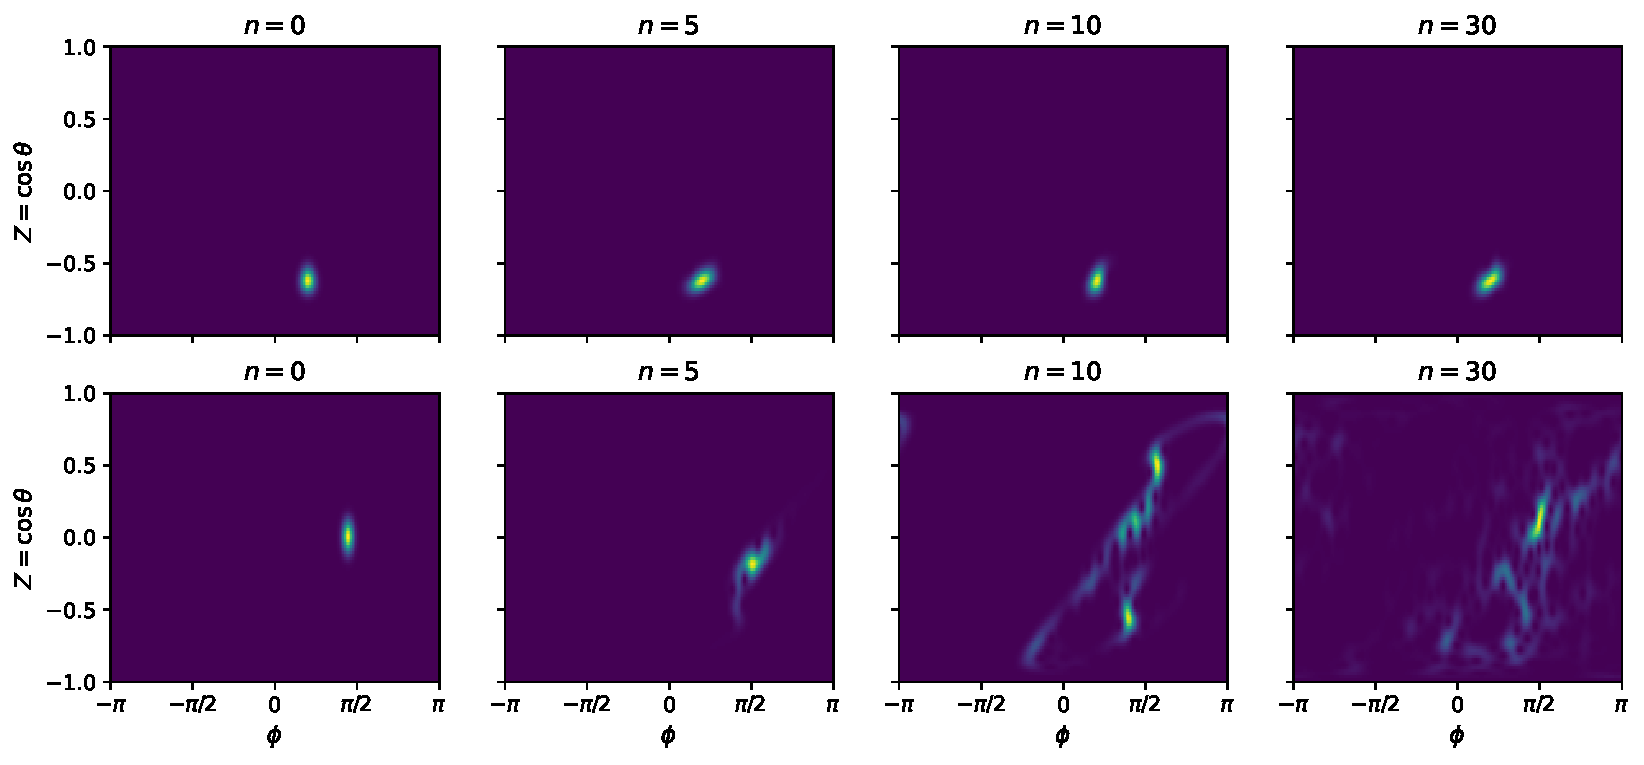
\includegraphics[width=\textwidth]{figures/quantum_husimi.pdf}
\caption{Husimi distribution \eqref{eq:husimi} of a coherent state, $j = 200$, $p = \pi/2$, $k = 3$, after $n = 0, 5,
10, 30$ kicks. Top: started in the regular island at $(\theta_0,\phi_0) = (2.25, 0.63)$, where it stays.
Bottom: started in the chaotic sea at $(\pi/2, 1.4)$, where it spreads over the chaotic region of
\cref{fig:portraits} and avoids the islands.}
\label{fig:quantum-husimi}
\end{figure}

\begin{figure}[h]
\centering
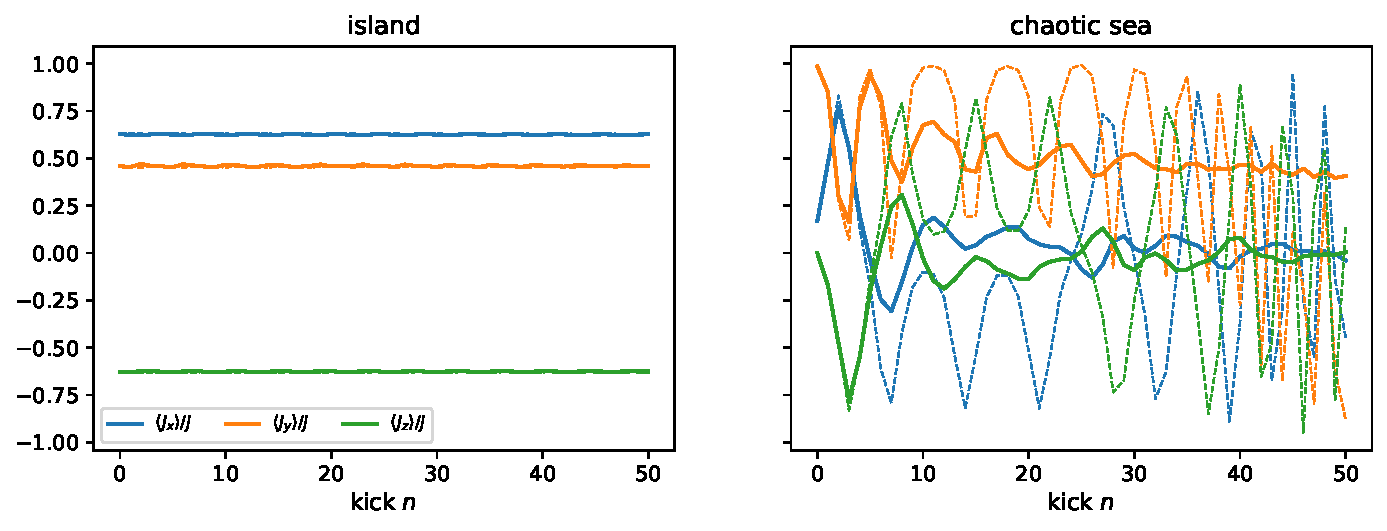
\includegraphics[width=\textwidth]{figures/quantum_expectation.pdf}
\caption{$\langle\hat{\vJ}\rangle/j$ (solid) and the classical orbit from the same point (dashed), $j = 200$, for the two
initial states of \cref{fig:quantum-husimi}. The island start lies close to the fixed point $\vs_+$
(\cref{sec:stability}), so both curves stay almost constant; in the chaotic sea they separate after a few kicks.}
\label{fig:quantum-expectation}
\end{figure}

\begin{figure}[h]
\centering
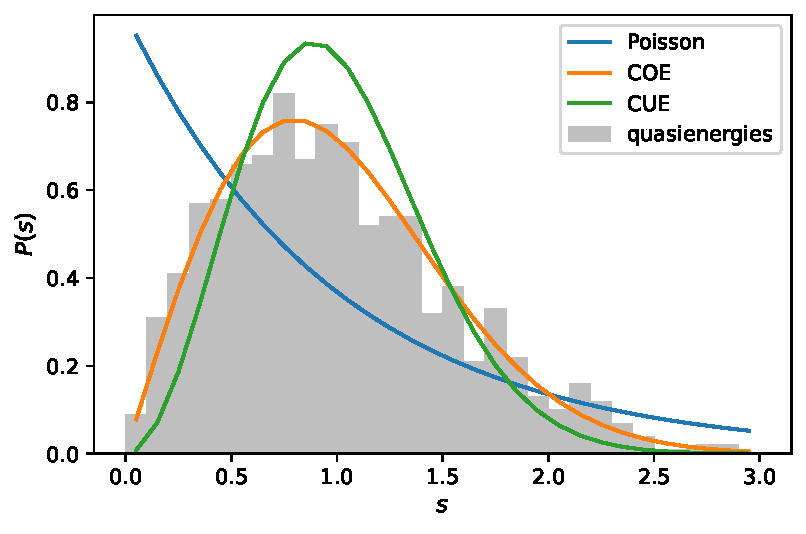
\includegraphics[width=0.6\textwidth]{figures/quantum_spacings.pdf}
\caption{Distribution of unfolded quasienergy spacings \eqref{eq:unfold}, both parity sectors, $j = 500$, $p = 1.7$,
$k = 10$, compared with \eqref{eq:wigner}.}
\label{fig:quantum-spacings}
\end{figure}


\begin{thebibliography}{9}
\bibitem{HKS1987} F.~Haake, M.~Ku\'s, R.~Scharf, \emph{Classical and quantum chaos for a kicked top},
  Z.~Phys.~B \textbf{65}, 381 (1987).
\bibitem{Haake} F.~Haake, S.~Gnutzmann, M.~Ku\'s, \emph{Quantum Signatures of Chaos}, 4th ed., Springer (2018).
\bibitem{LL} A.~J.~Lichtenberg, M.~A.~Lieberman, \emph{Regular and Chaotic Dynamics}, 2nd ed., Springer (1992).
\bibitem{Ott} E.~Ott, \emph{Chaos in Dynamical Systems}, 2nd ed., Cambridge University Press (2002).
\bibitem{Arnold} V.~I.~Arnold, \emph{Mathematical Methods of Classical Mechanics}, 2nd ed., Springer (1989).
\bibitem{Chirikov} B.~V.~Chirikov, \emph{A universal instability of many-dimensional oscillator systems},
  Phys.~Rep.~\textbf{52}, 263 (1979).
\bibitem{Benettin} G.~Benettin, L.~Galgani, A.~Giorgilli, J.-M.~Strelcyn, \emph{Lyapunov characteristic exponents
  for smooth dynamical systems and for Hamiltonian systems}, Meccanica \textbf{15}, 9 (1980).
\bibitem{Chaudhury2009} S.~Chaudhury, A.~Smith, B.~E.~Anderson, S.~Ghose, P.~S.~Jessen, \emph{Quantum signatures of
  chaos in a kicked top}, Nature \textbf{461}, 768 (2009).
\bibitem{Neill2016} C.~Neill \emph{et al.}, \emph{Ergodic dynamics and thermalization in an isolated quantum
  system}, Nature Phys.~\textbf{12}, 1037 (2016).
\bibitem{Atas2013} Y.~Y.~Atas, E.~Bogomolny, O.~Giraud, G.~Roux, \emph{Distribution of the ratio of consecutive level
spacings in random matrix ensembles}, Phys. Rev. Lett. \textbf{110}, 084101 (2013).
\end{thebibliography}

\end{document}
